% ============================================================
%  第六章：实验评估
% ============================================================
\section{实验评估}

% ---- Slide: 实验设置 ----
\begin{frame}{实验设置}

  \begin{columns}[T]
    \column{0.48\textwidth}
      \begin{block}{硬件与实现}
        \begin{itemize}
          \item \textbf{平台}：Apple M1 · 8 核 CPU · 16\,GB 内存
          \item \textbf{语言}：C++11
          \item \textbf{密码库}：OpenSSL（SHA-256 / HMAC）、
                RELIC（配对运算）、Ed25519（数字签名）
          \item \textbf{基线}：Nomos、MC-ODXT
        \end{itemize}
      \end{block}

    \column{0.48\textwidth}
      \begin{block}{数据集}
        \small
        \begin{tabular}{lccc}
          \toprule
          \textbf{数据集} & \textbf{关键词对} & \textbf{不同关键词} & \textbf{最高频} \\
          \midrule
          Crime   & 7,989,987 & 63,659 & 16,644 \\
          Enron   & 5,190,199 & 16,241 & 26,946 \\
          Wiki    & 4,565,948 & 10,000 &  9,738 \\
          \bottomrule
        \end{tabular}
      \end{block}
  \end{columns}

  \vspace{0.4em}
  \begin{exampleblock}{评估维度}
    更新/搜索时间（客户端、授权管理方、服务器）
    $\cdot$ 客户端/服务器存储
    $\cdot$ 通信开销
    $\cdot$ 验证开销随候选集规模 $m$ 的变化
  \end{exampleblock}

\end{frame}

% ---- Slide: 搜索时间——客户端 ----
\begin{frame}{实验结果（一）：客户端搜索时间}

  \begin{figure}
    \begin{subfigure}[b]{0.32\textwidth}
      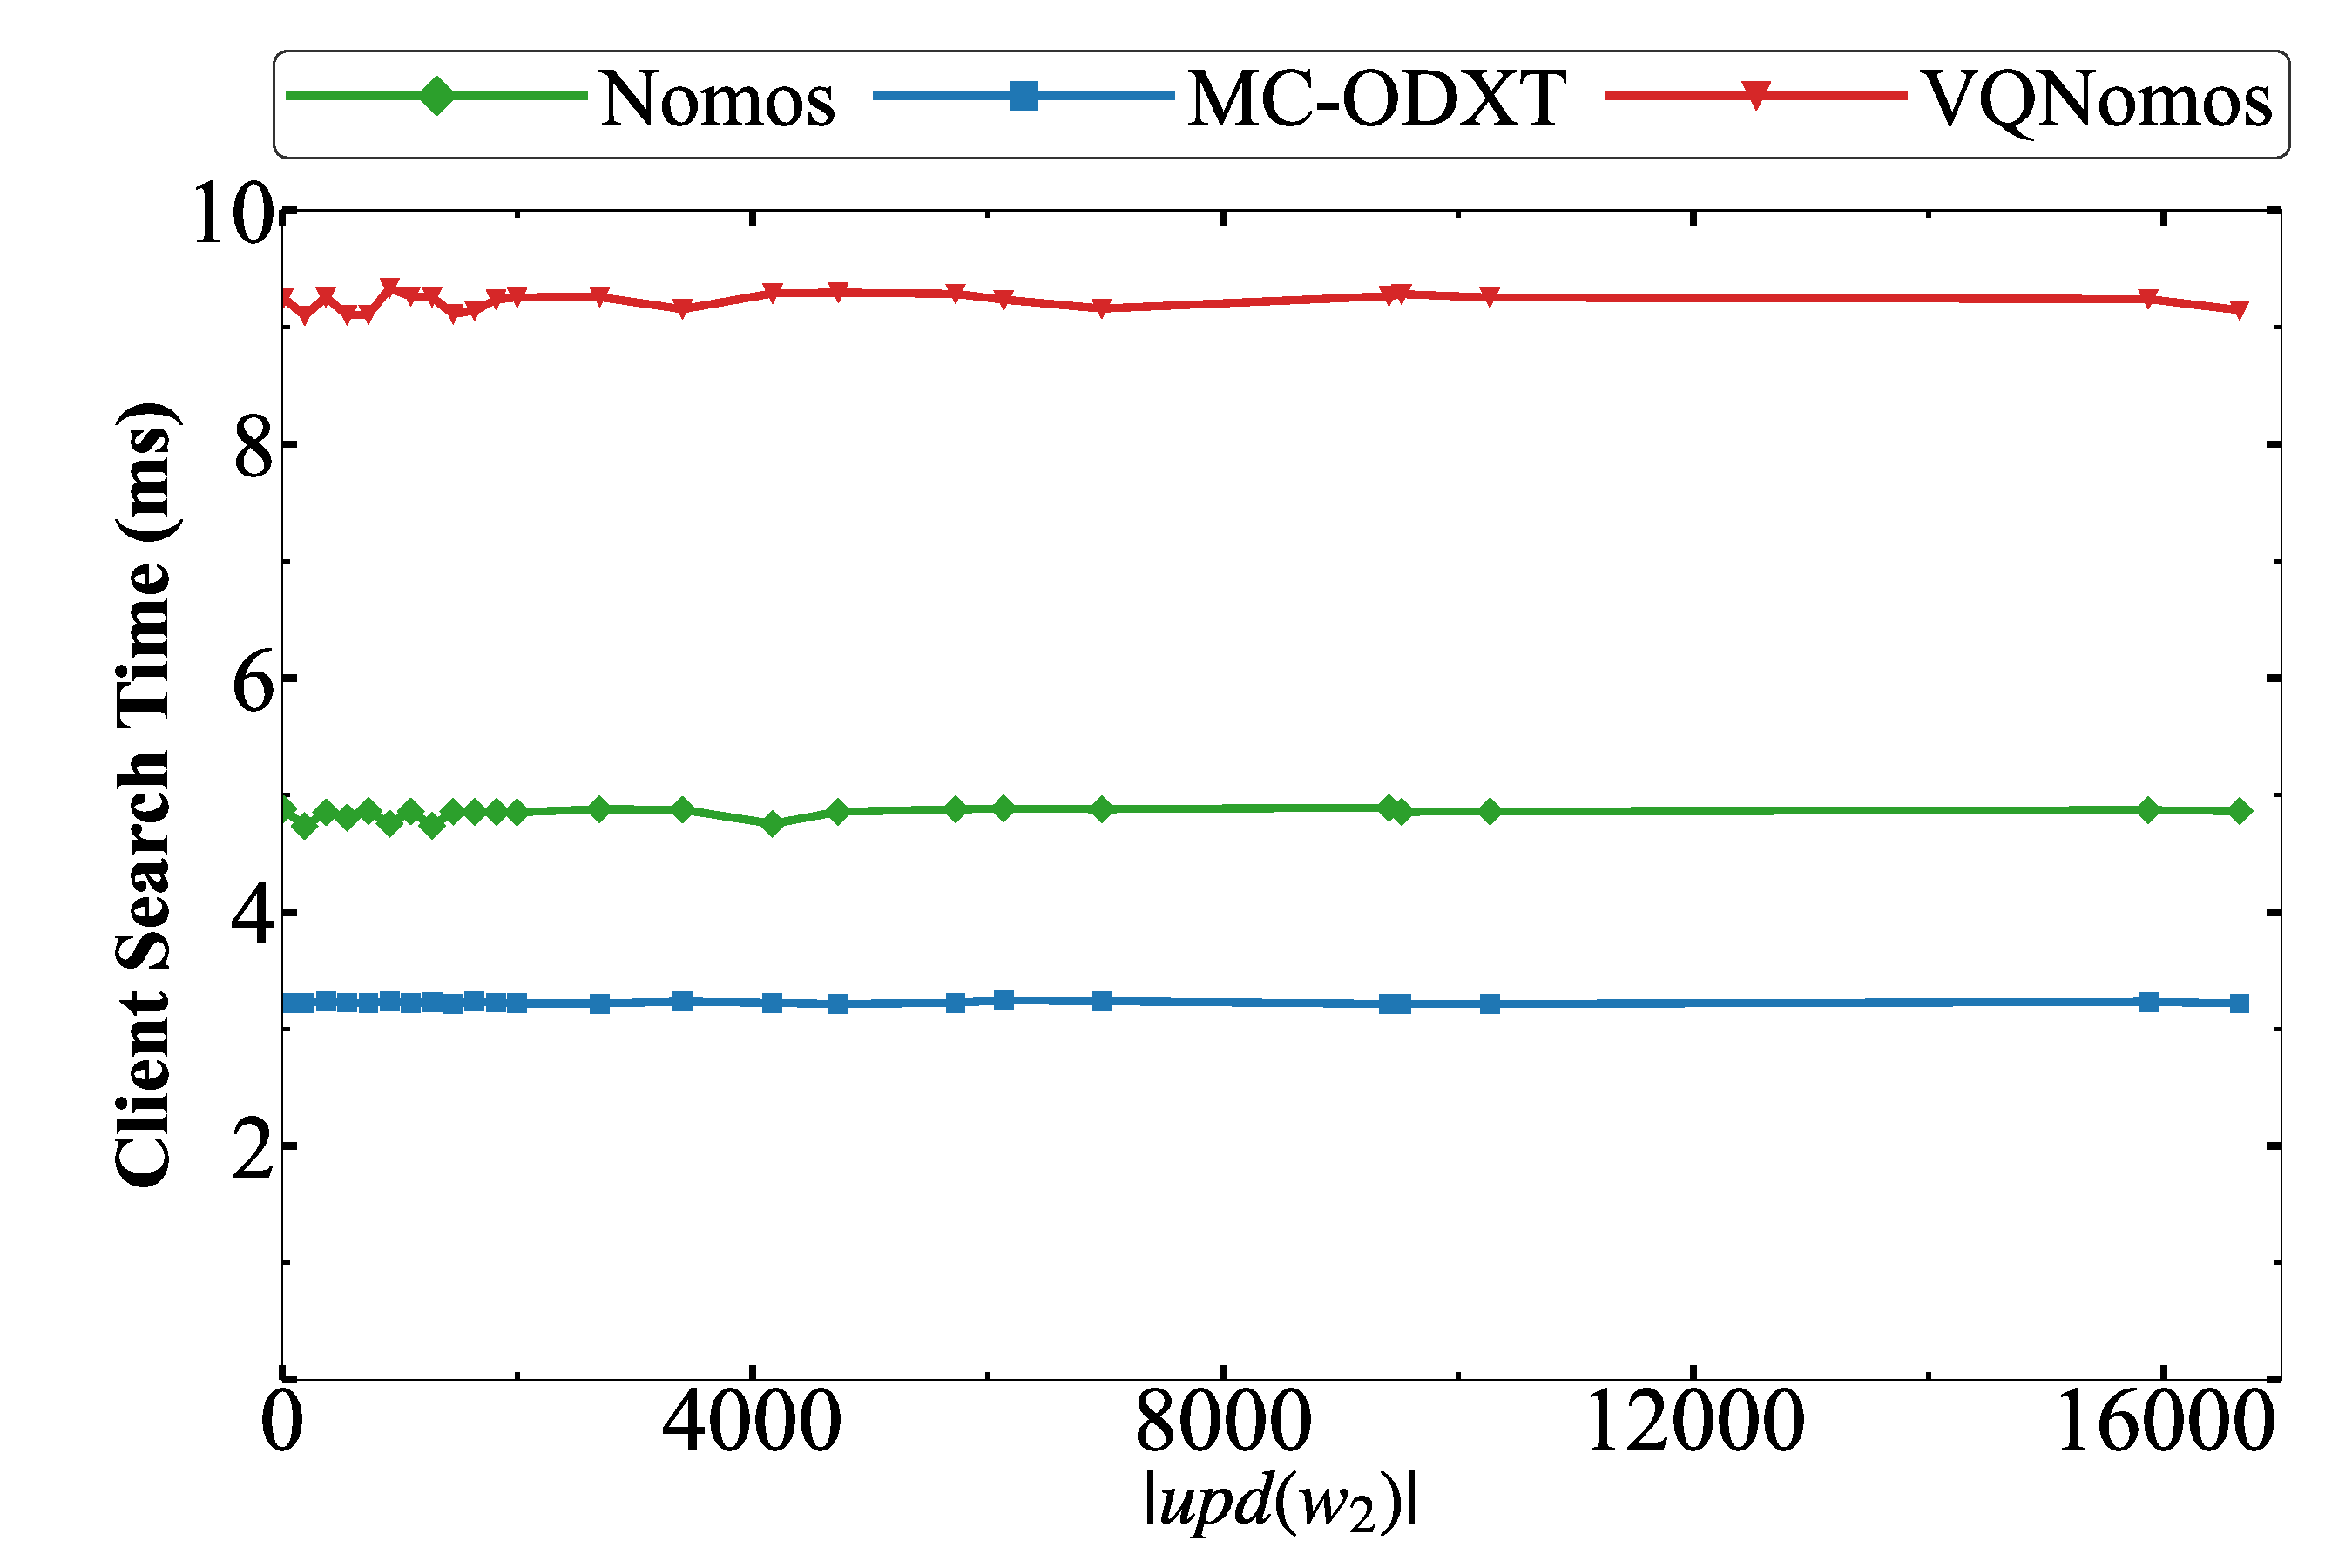
\includegraphics[width=\linewidth]
        {../figures/client_search_time_fixed_w1_figures/Crime_client_search_time_comparison.pdf}
      \caption{Crime}
    \end{subfigure}
    \hfill
    \begin{subfigure}[b]{0.32\textwidth}
      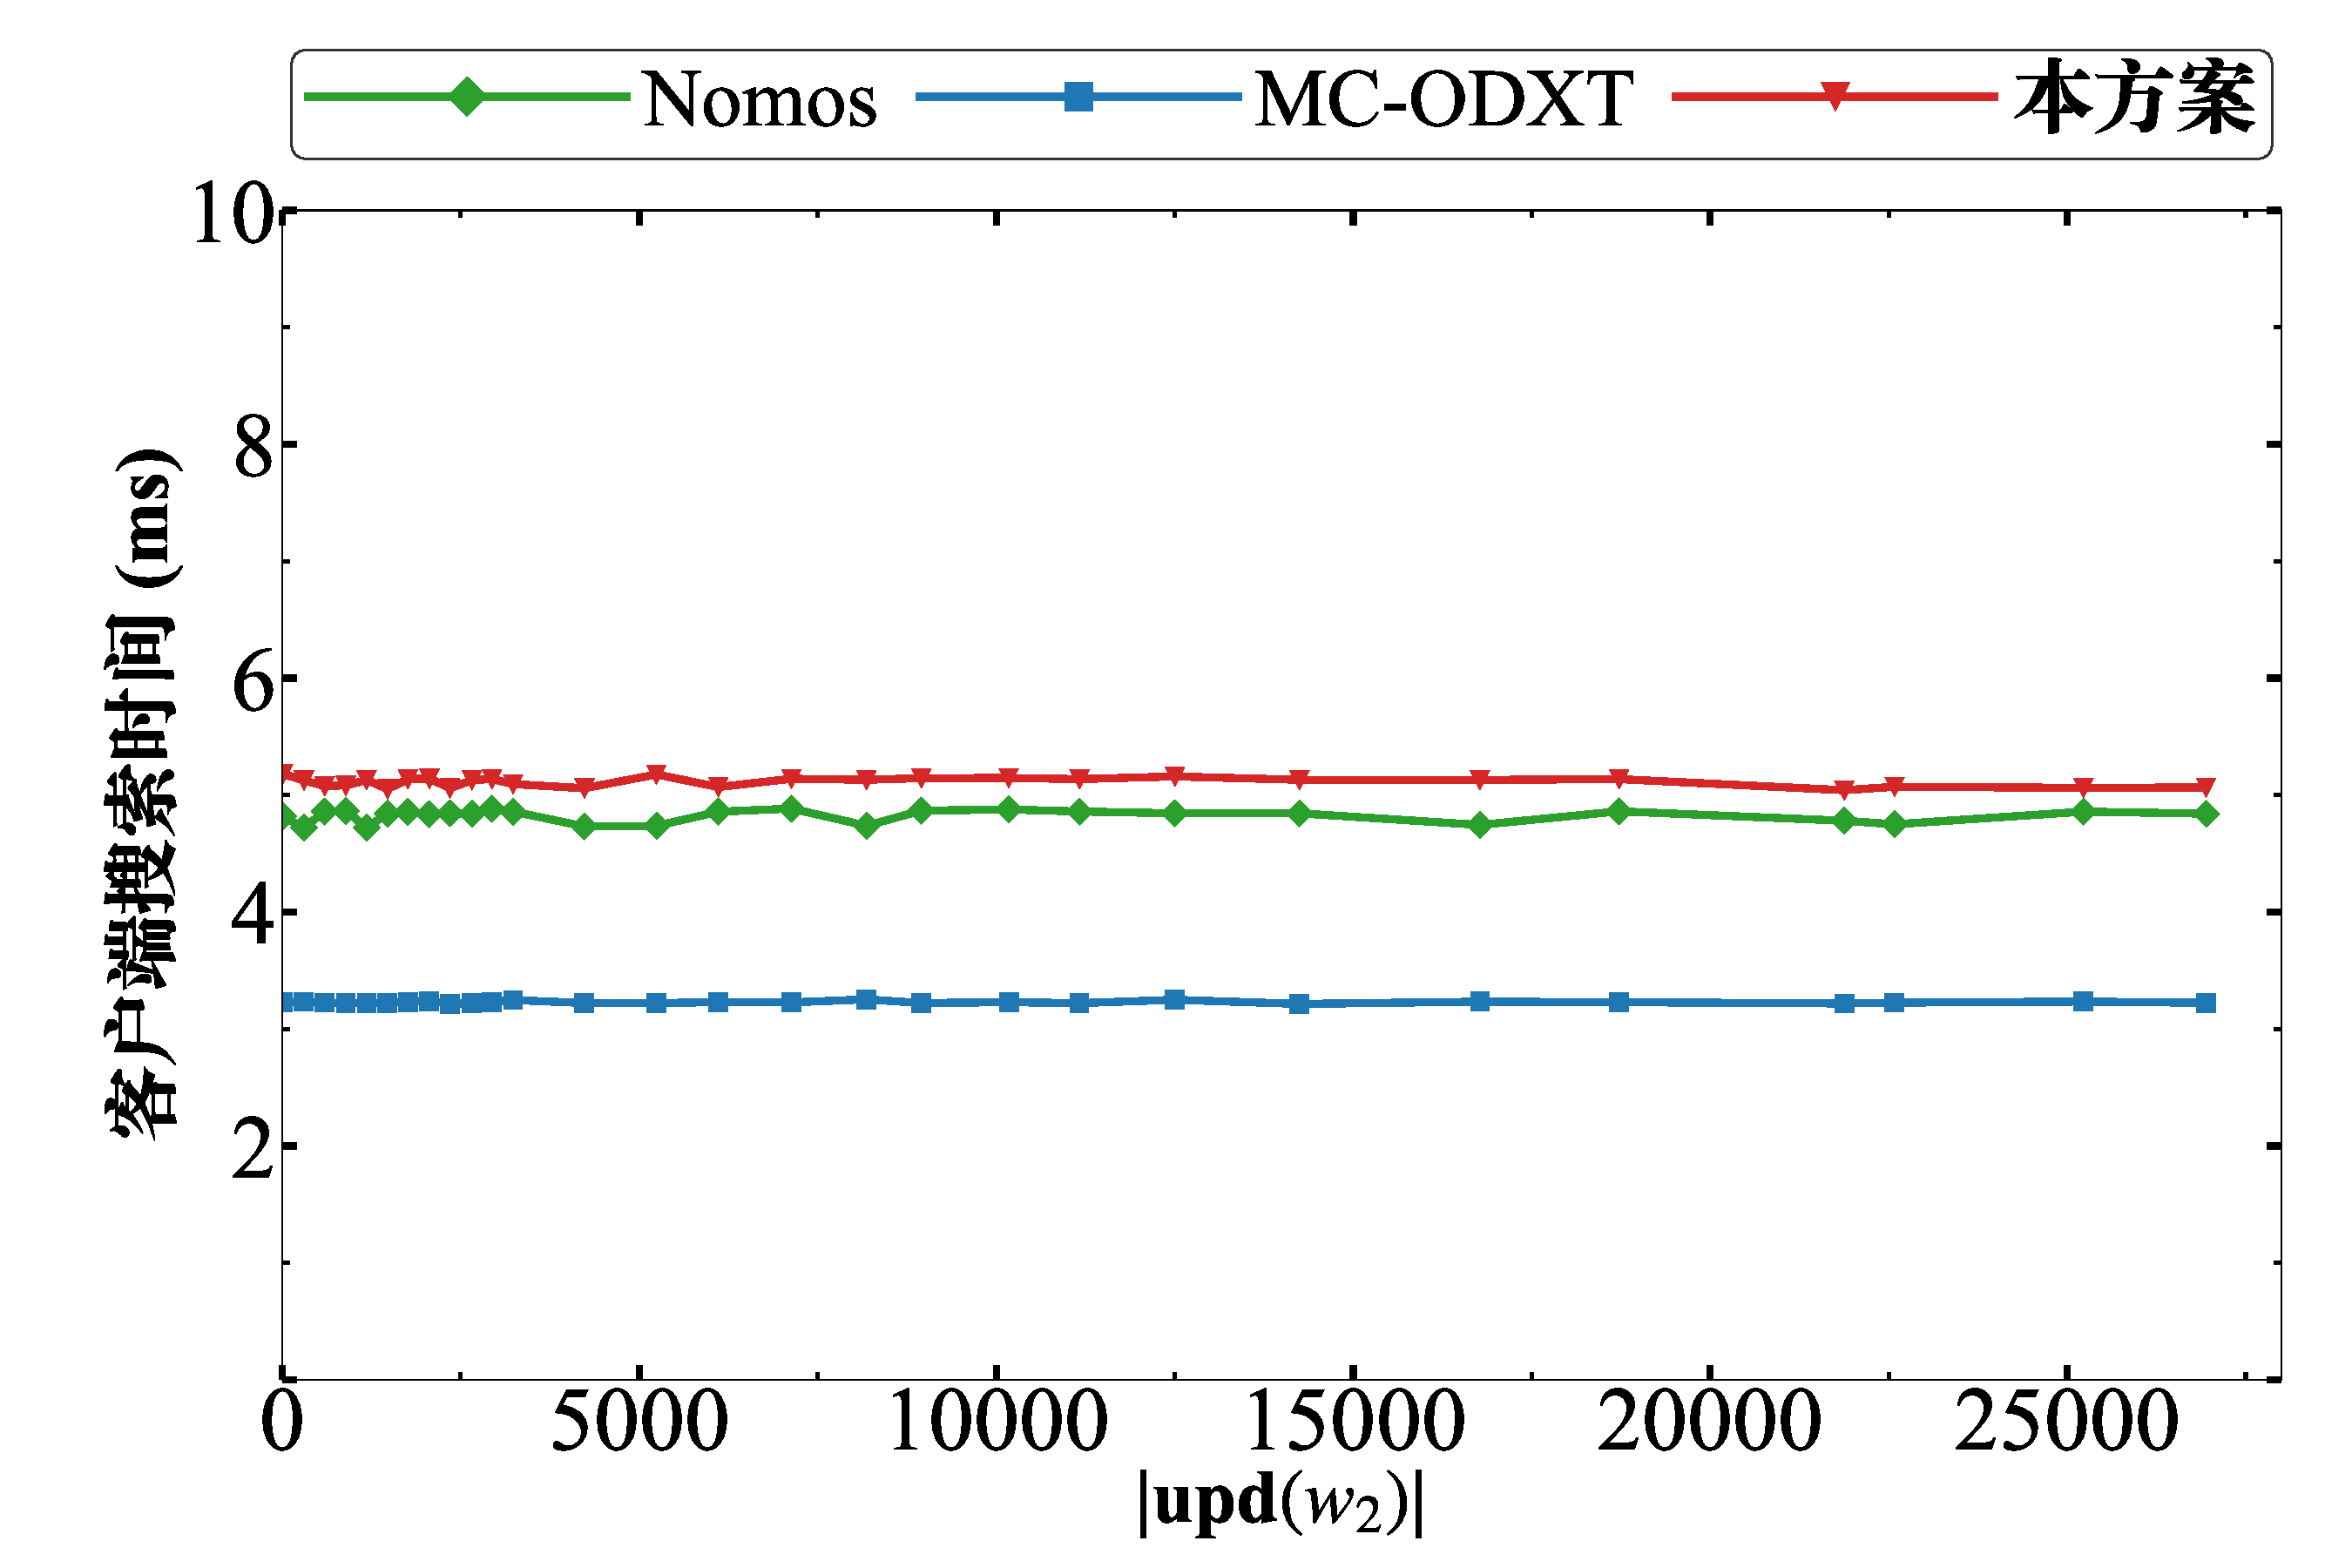
\includegraphics[width=\linewidth]
        {../figures/client_search_time_fixed_w1_figures/Enron_client_search_time_comparison.pdf}
      \caption{Enron}
    \end{subfigure}
    \hfill
    \begin{subfigure}[b]{0.32\textwidth}
      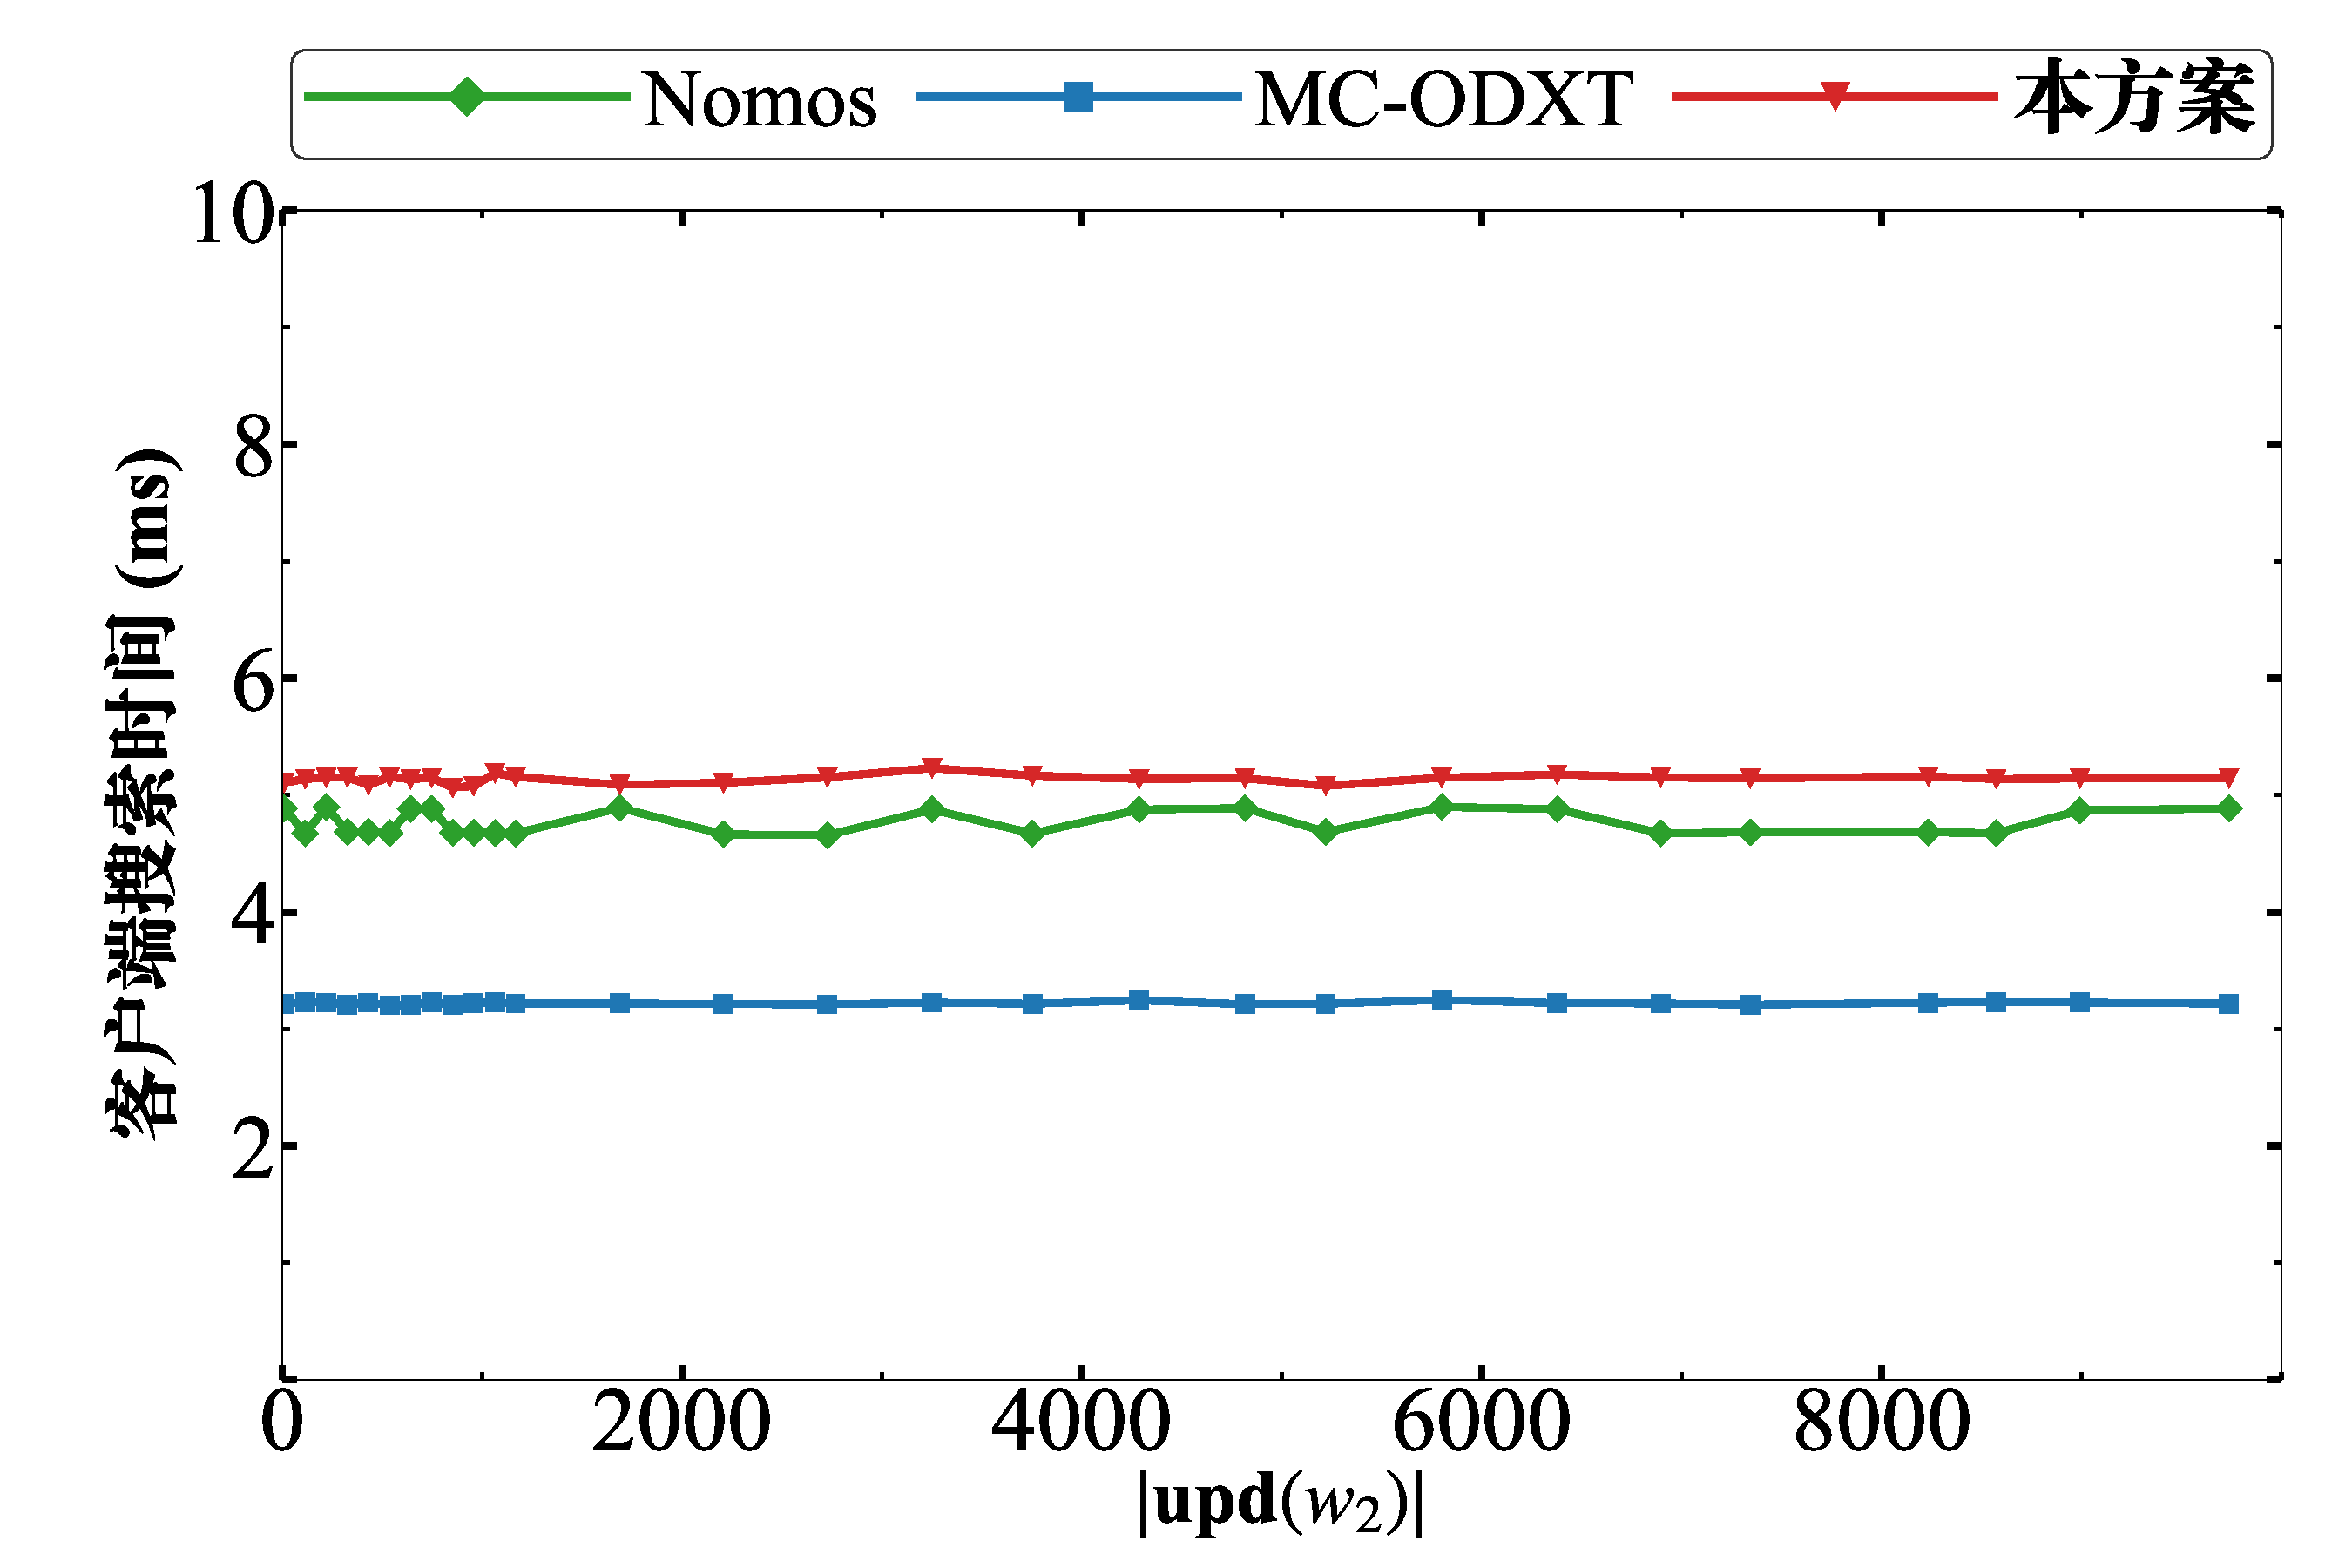
\includegraphics[width=\linewidth]
        {../figures/client_search_time_fixed_w1_figures/Wikipedia_client_search_time_comparison.pdf}
      \caption{Wiki}
    \end{subfigure}
    \caption{客户端搜索时间（与 Nomos 基线对比）}
  \end{figure}

  \begin{exampleblock}{核心结论}
    客户端搜索时间增量 $< 10\%$；
    授权管理方增量 $< 5\%$；
    搜索时间随候选集大小 $m$ 线性增长，
    符合 $O(k|Q| \cdot \mathsf{UpdateCnt}[w_s])$ 理论预测。
  \end{exampleblock}

\end{frame}

% ---- Slide: 搜索时间——服务器与管理方 ----
\begin{frame}{实验结果（二）：服务器与授权管理方搜索时间}

  \begin{columns}[T]
    \column{0.50\textwidth}
      \begin{figure}
        \begin{subfigure}[b]{0.49\textwidth}
          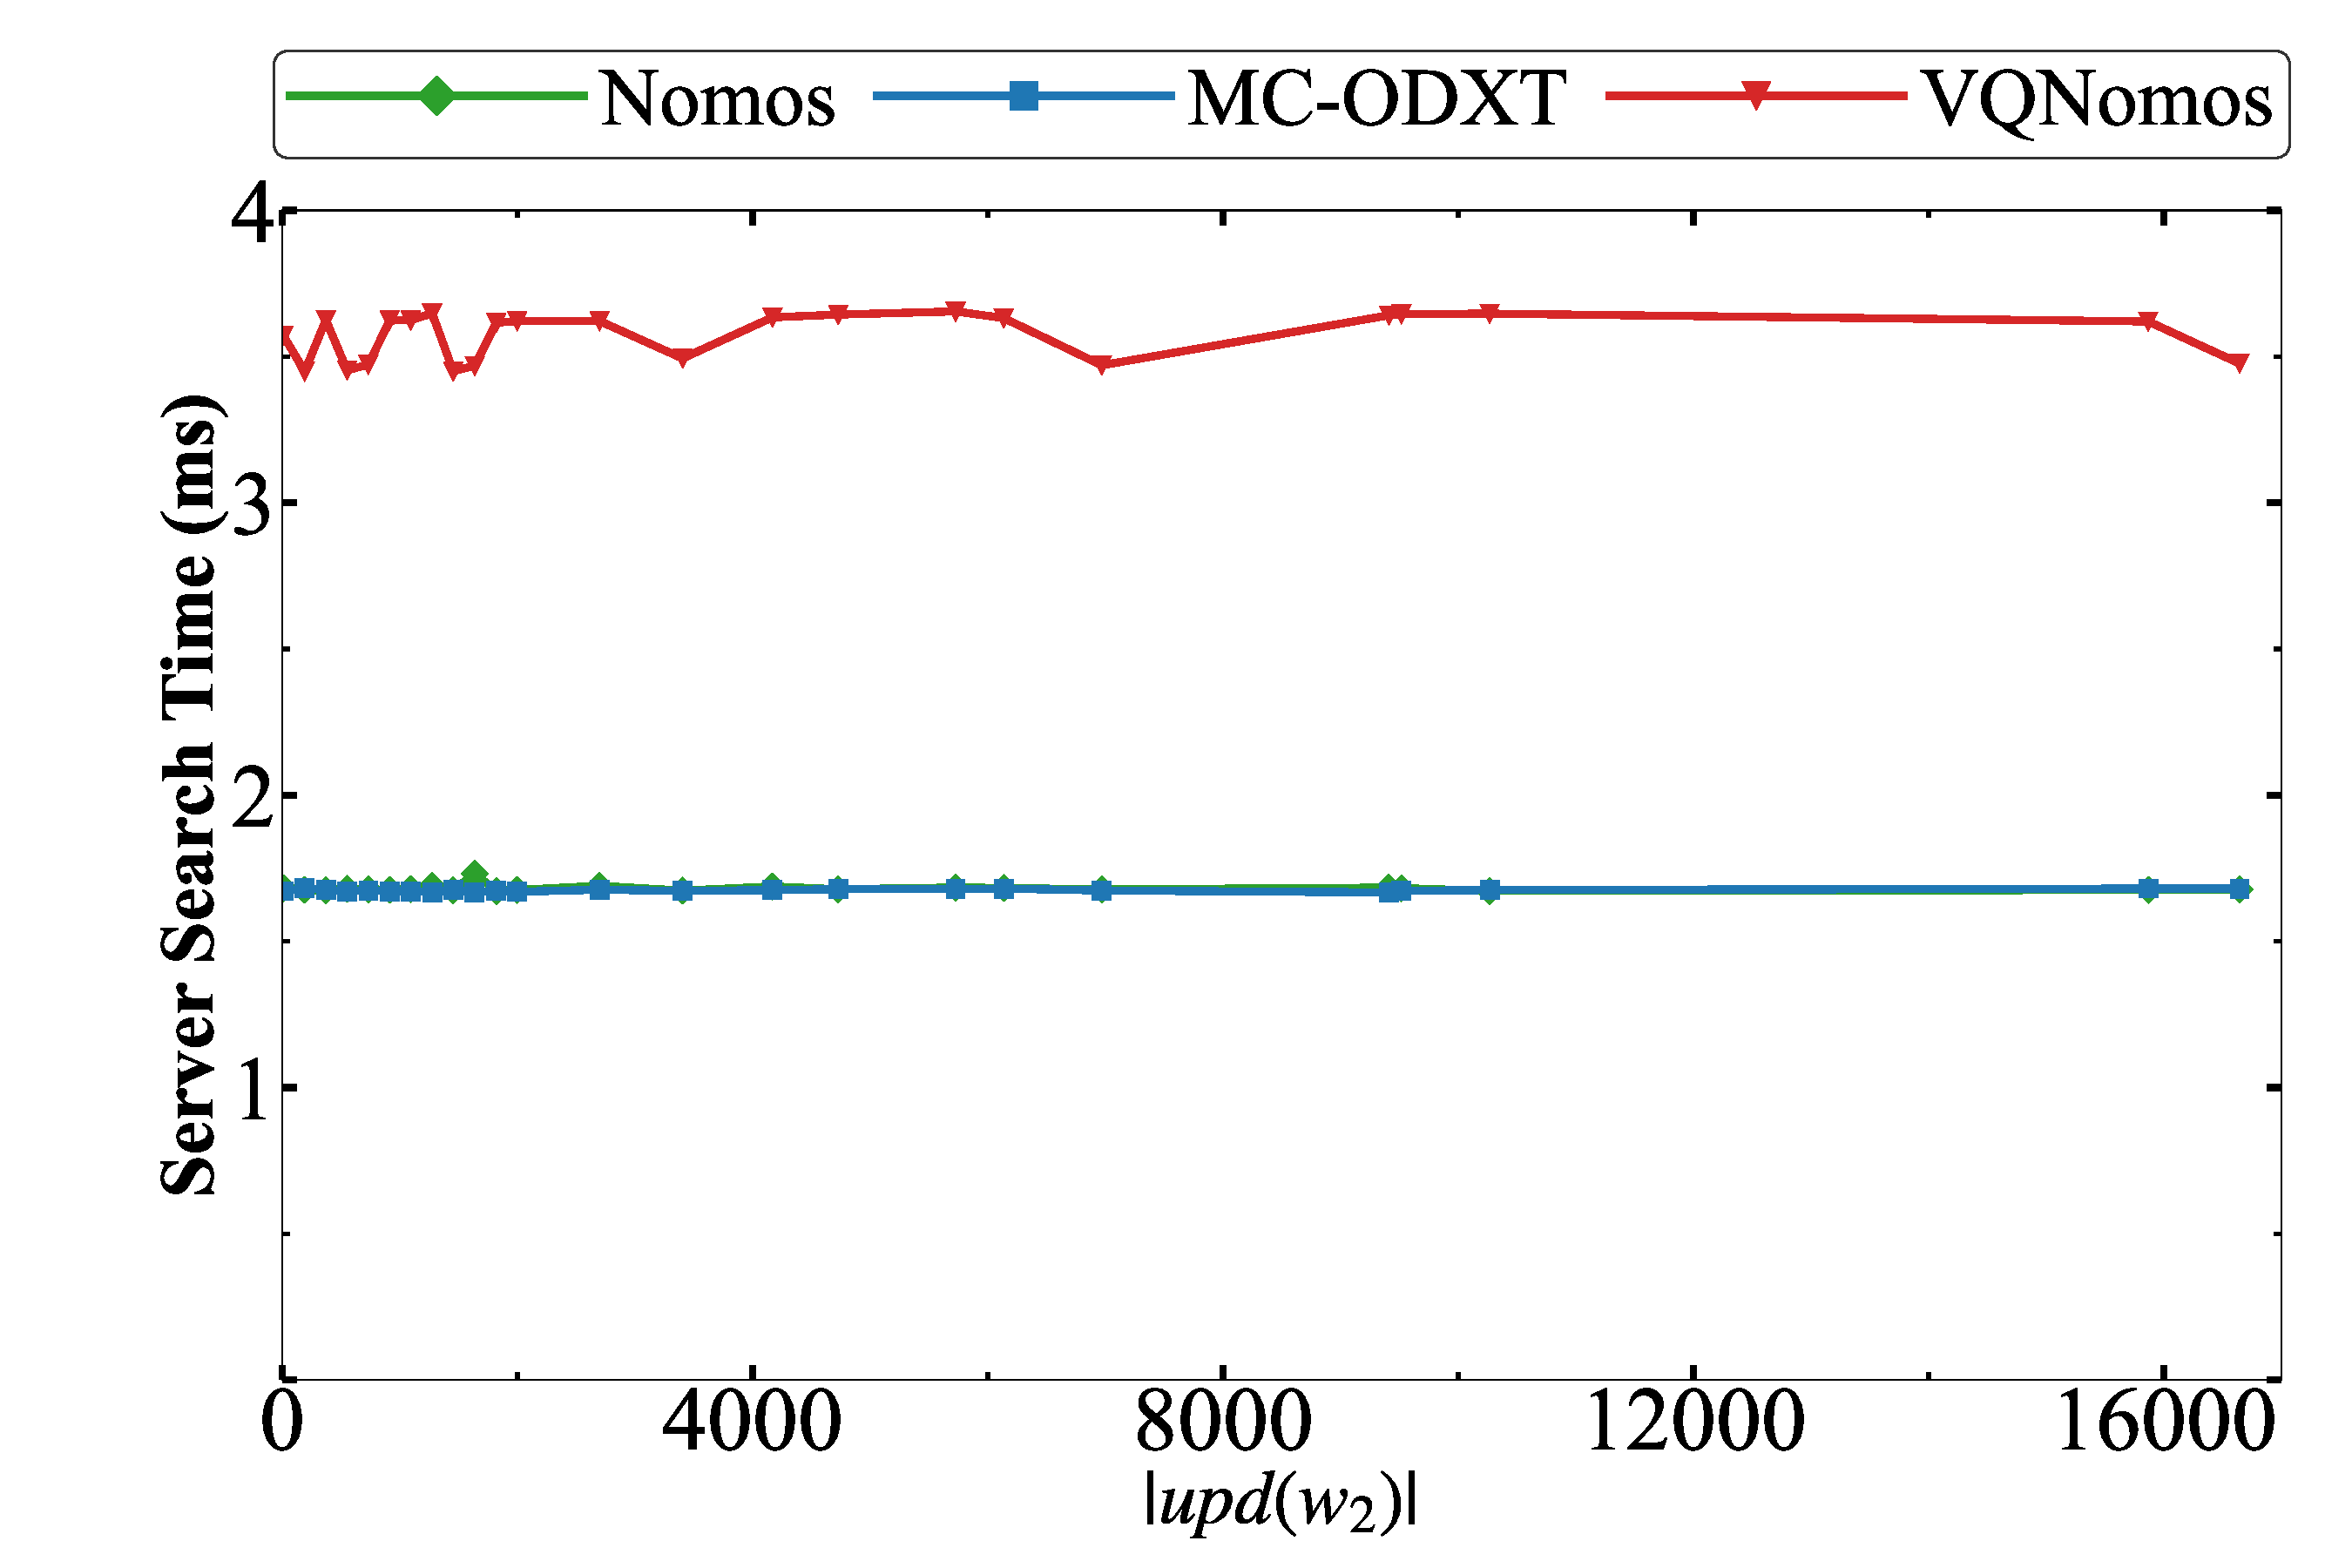
\includegraphics[width=\linewidth]
            {../figures/server_search_time_fixed_w1_figures/Crime_server_search_time_comparison.pdf}
        \end{subfigure}
        \hfill
        \begin{subfigure}[b]{0.49\textwidth}
          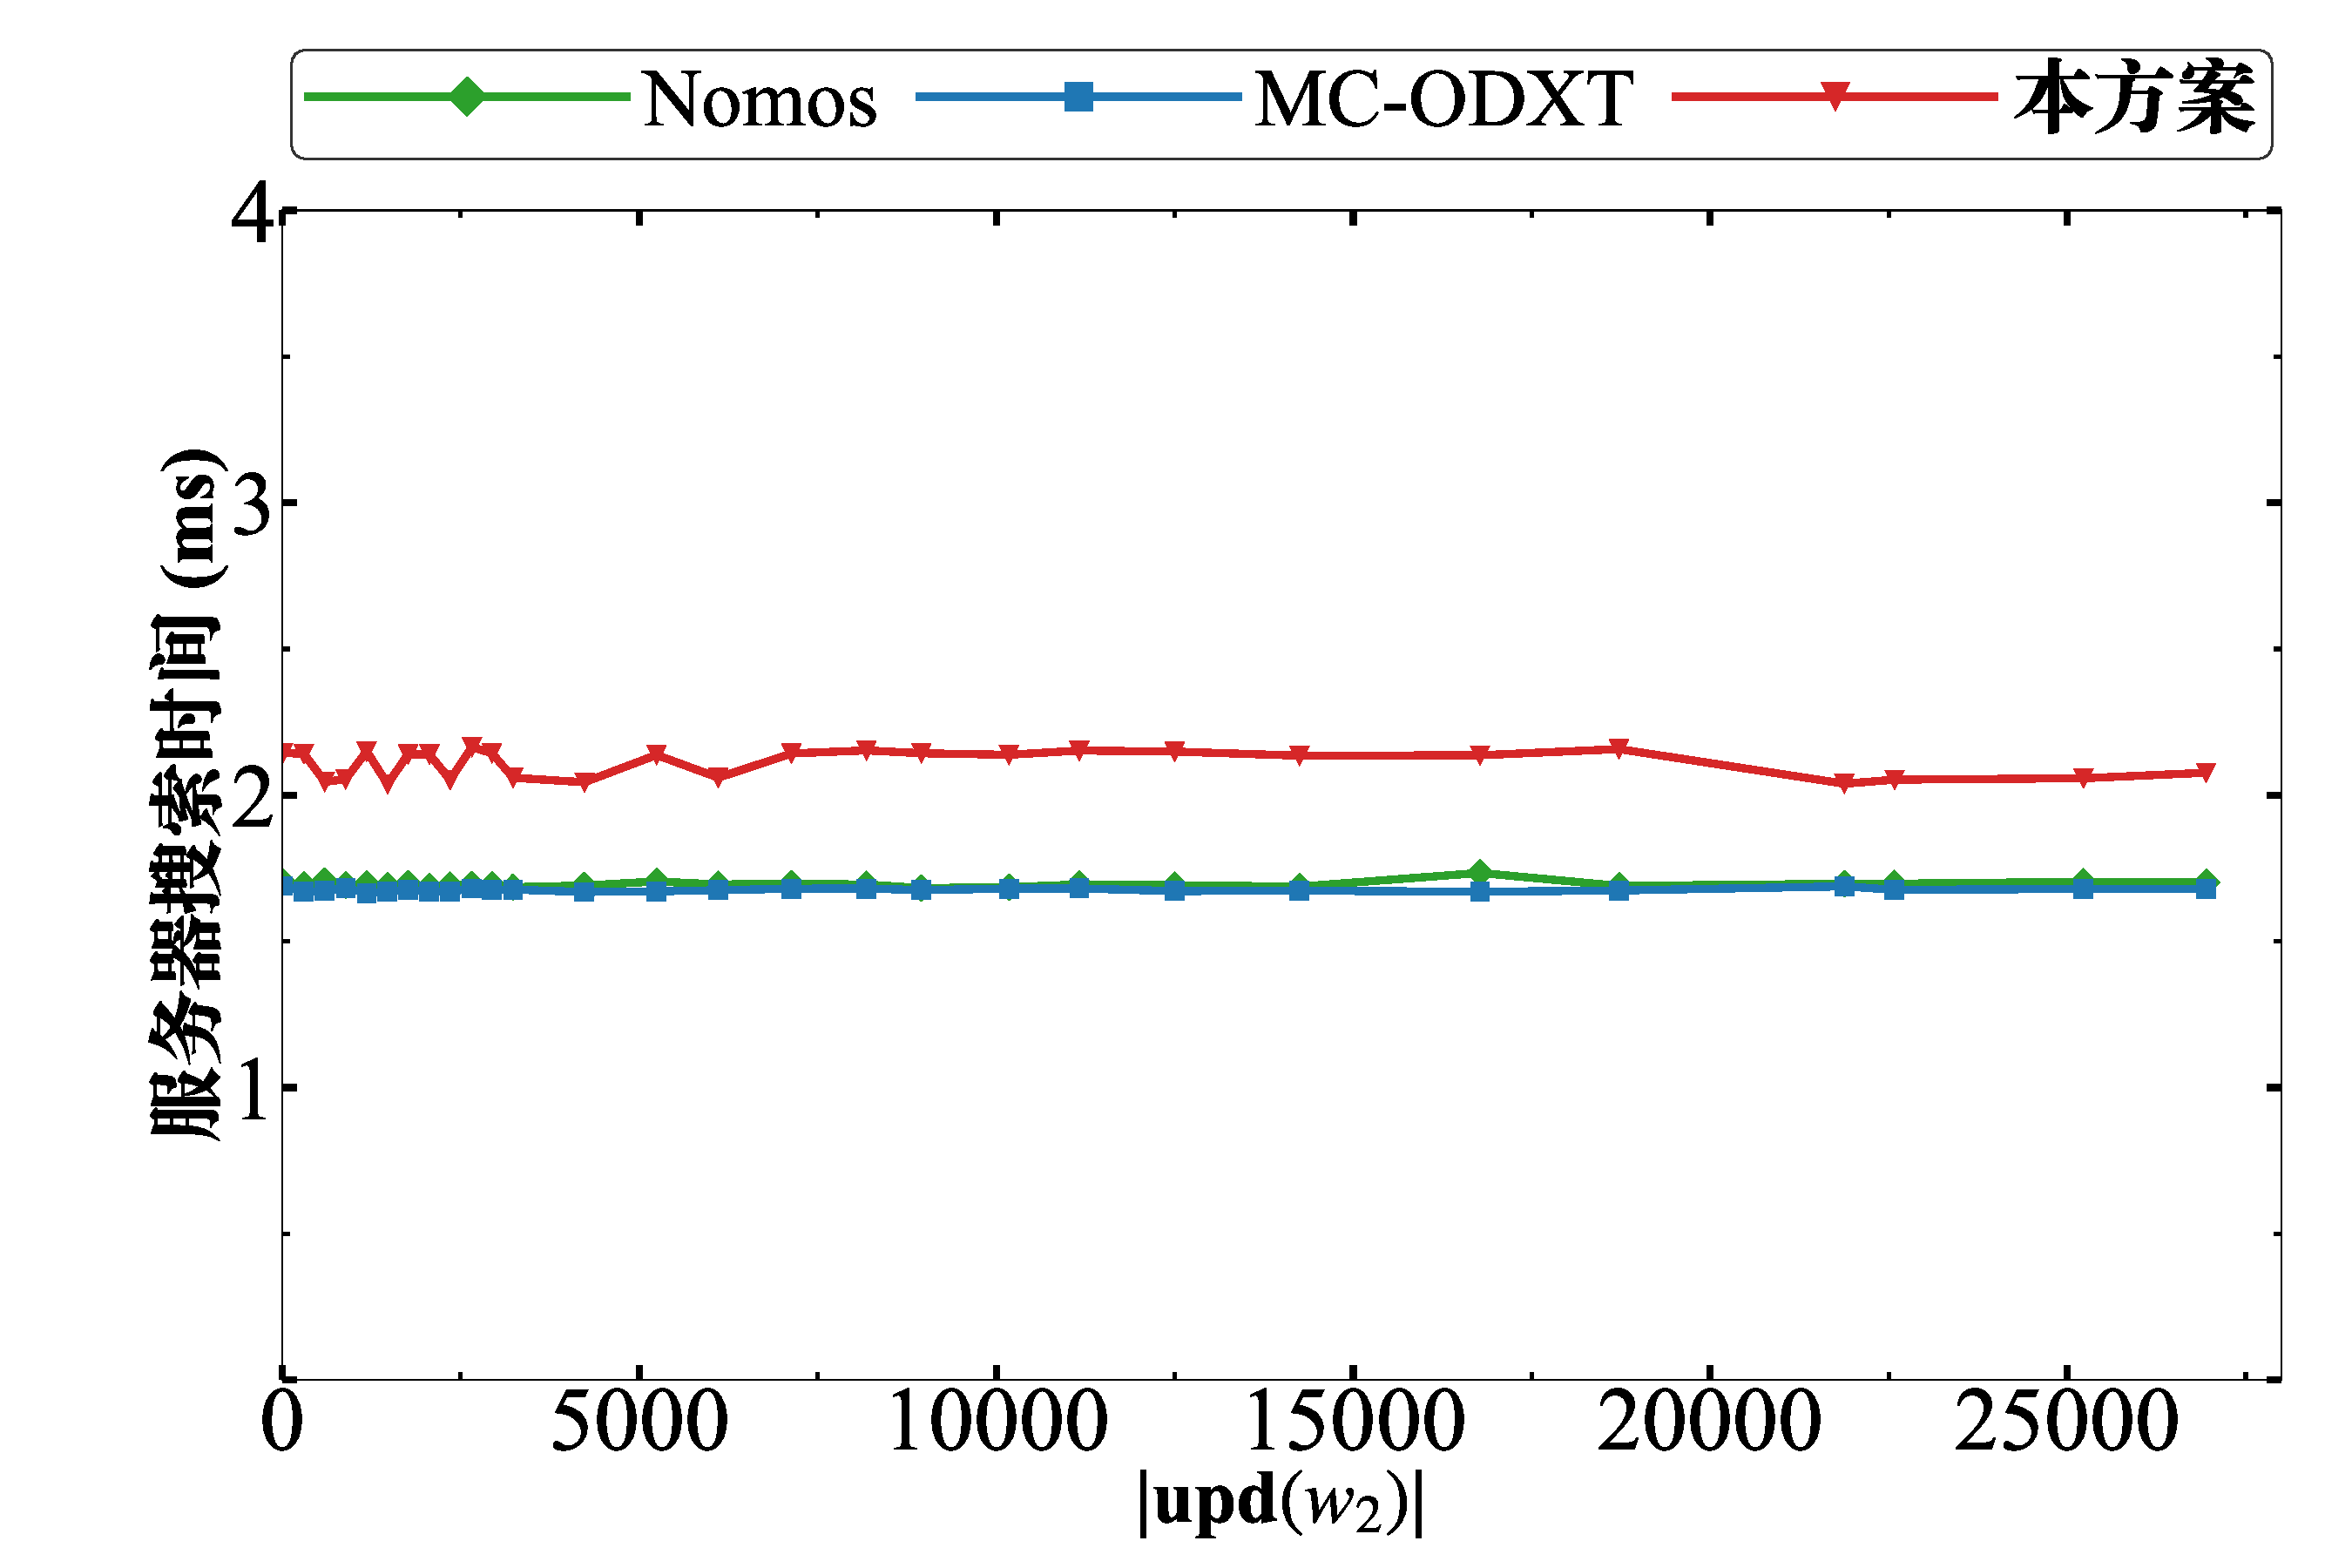
\includegraphics[width=\linewidth]
            {../figures/server_search_time_fixed_w1_figures/Enron_server_search_time_comparison.pdf}
        \end{subfigure}
        \caption{服务器搜索时间}
      \end{figure}

    \column{0.47\textwidth}
      \begin{figure}
        \begin{subfigure}[b]{0.49\textwidth}
          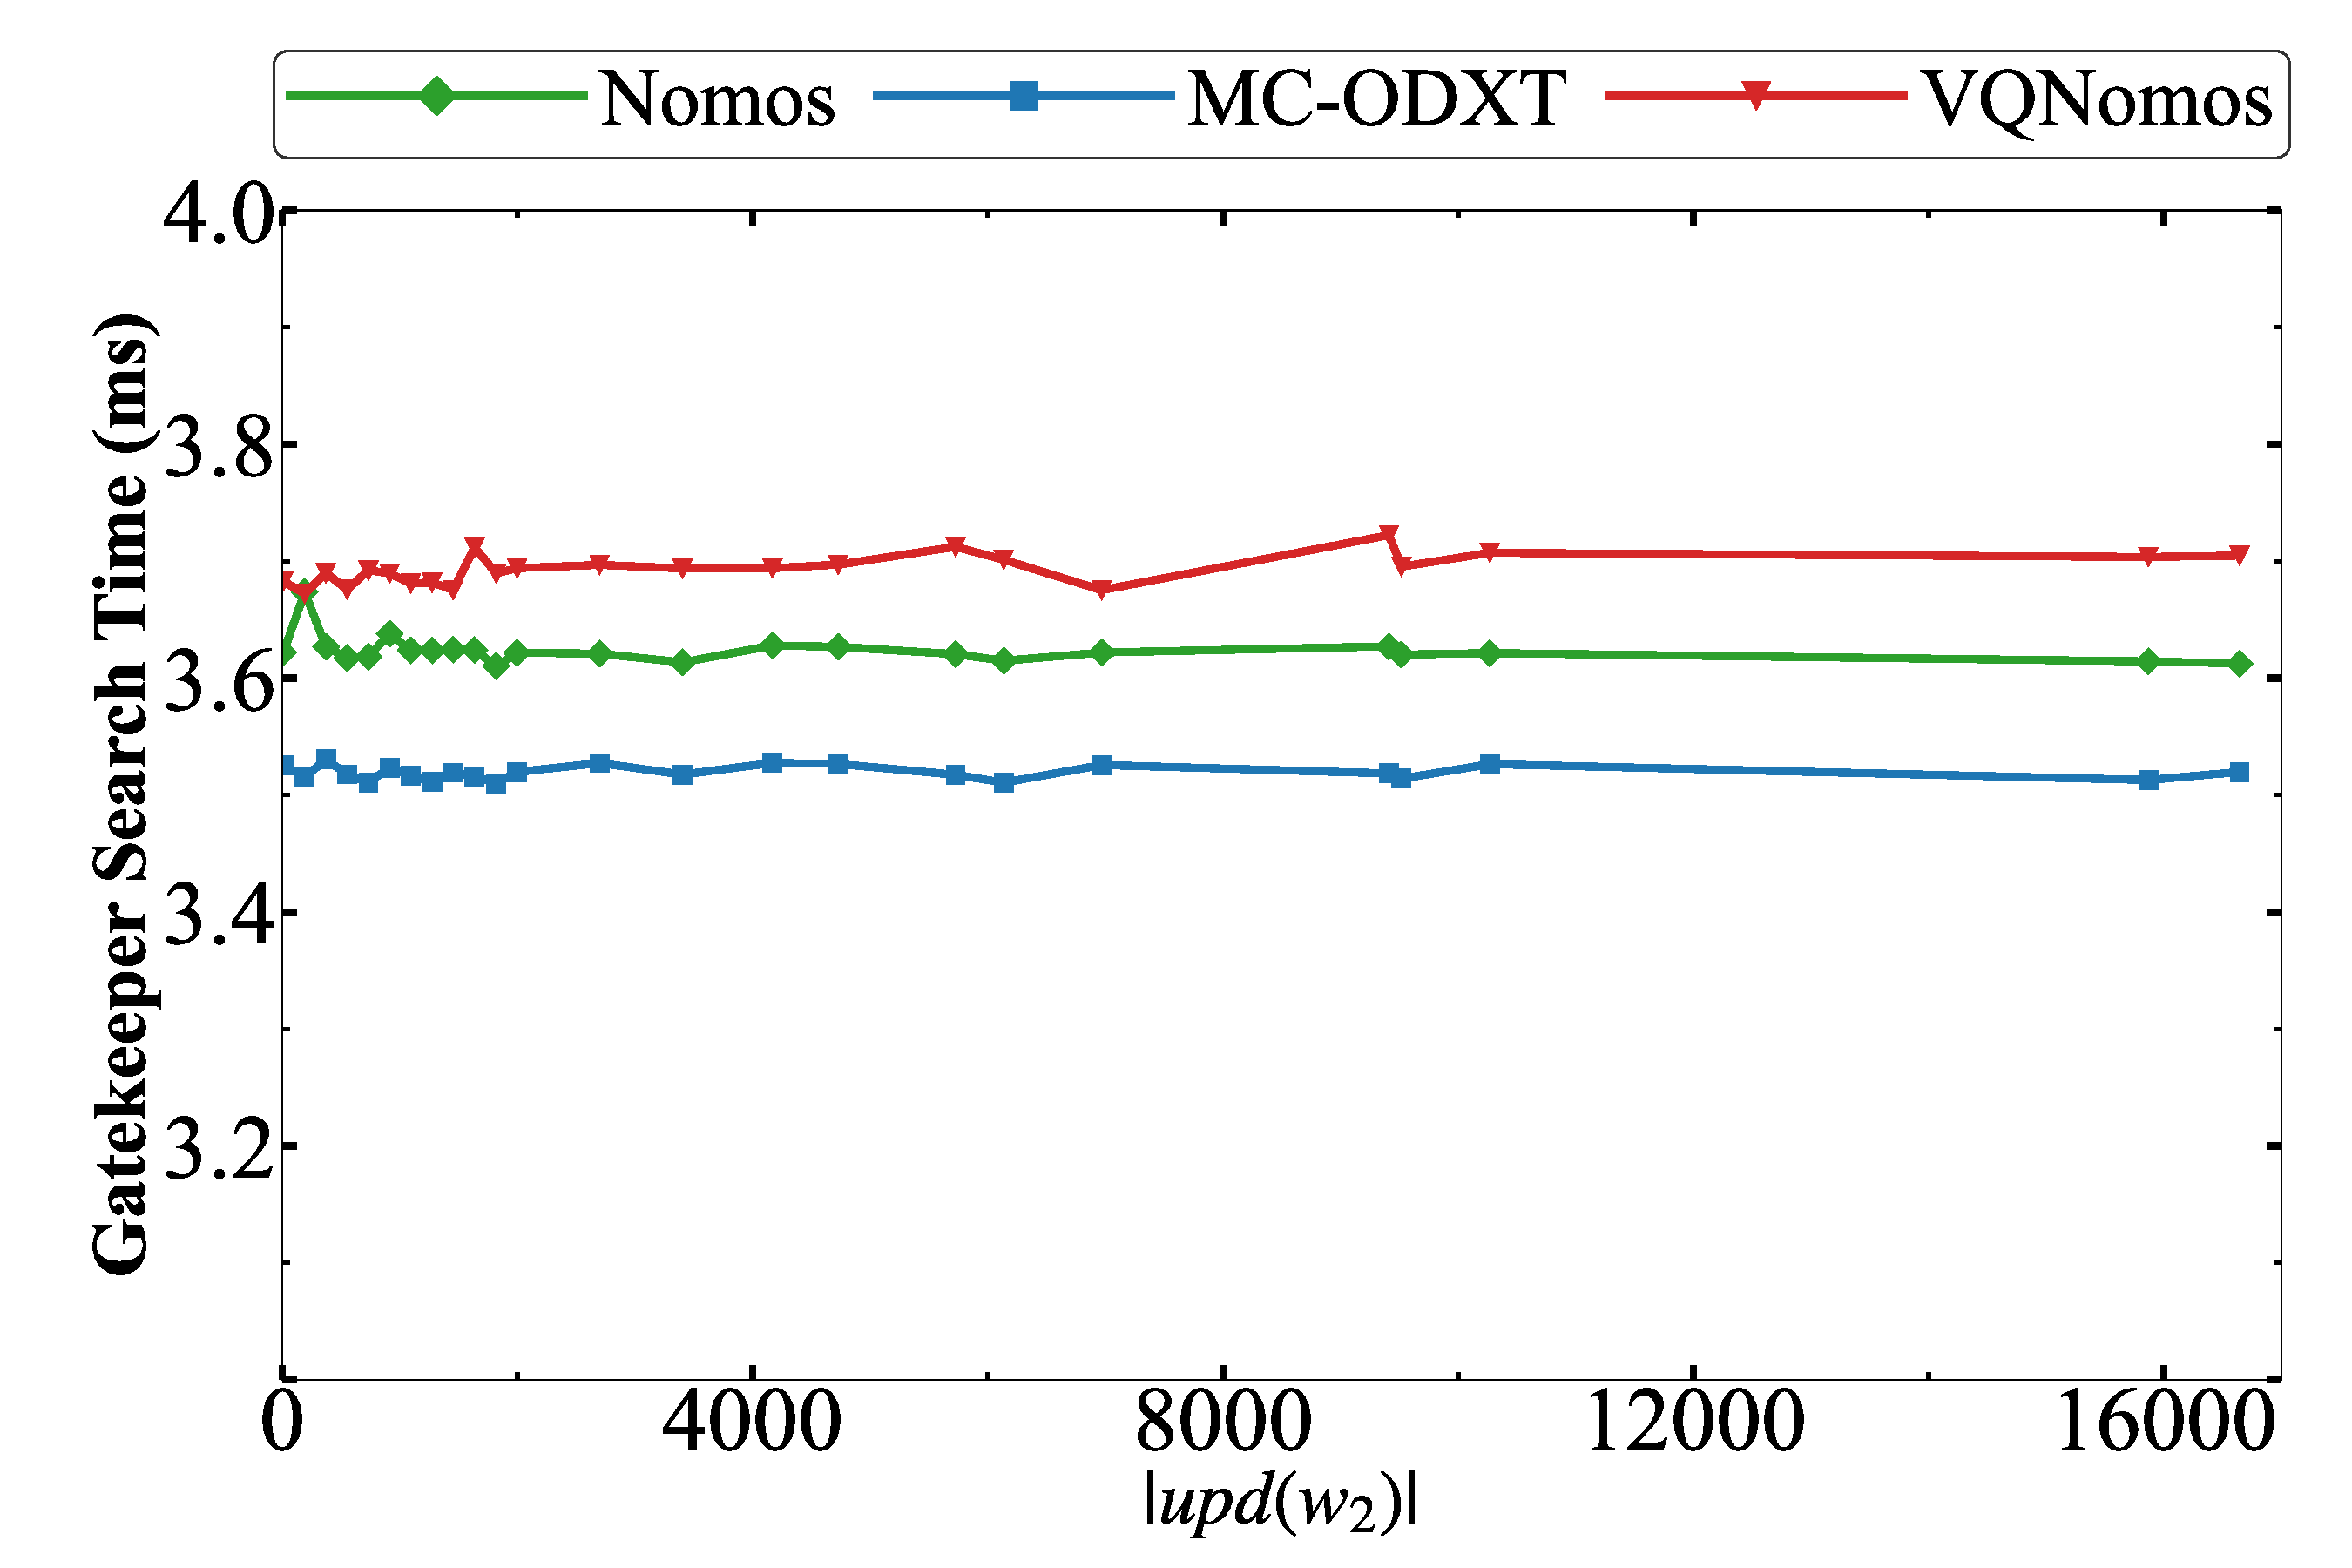
\includegraphics[width=\linewidth]
            {../figures/gatekeeper_search_time_fixed_w1_figures/Crime_gatekeeper_search_time_comparison.pdf}
        \end{subfigure}
        \hfill
        \begin{subfigure}[b]{0.49\textwidth}
          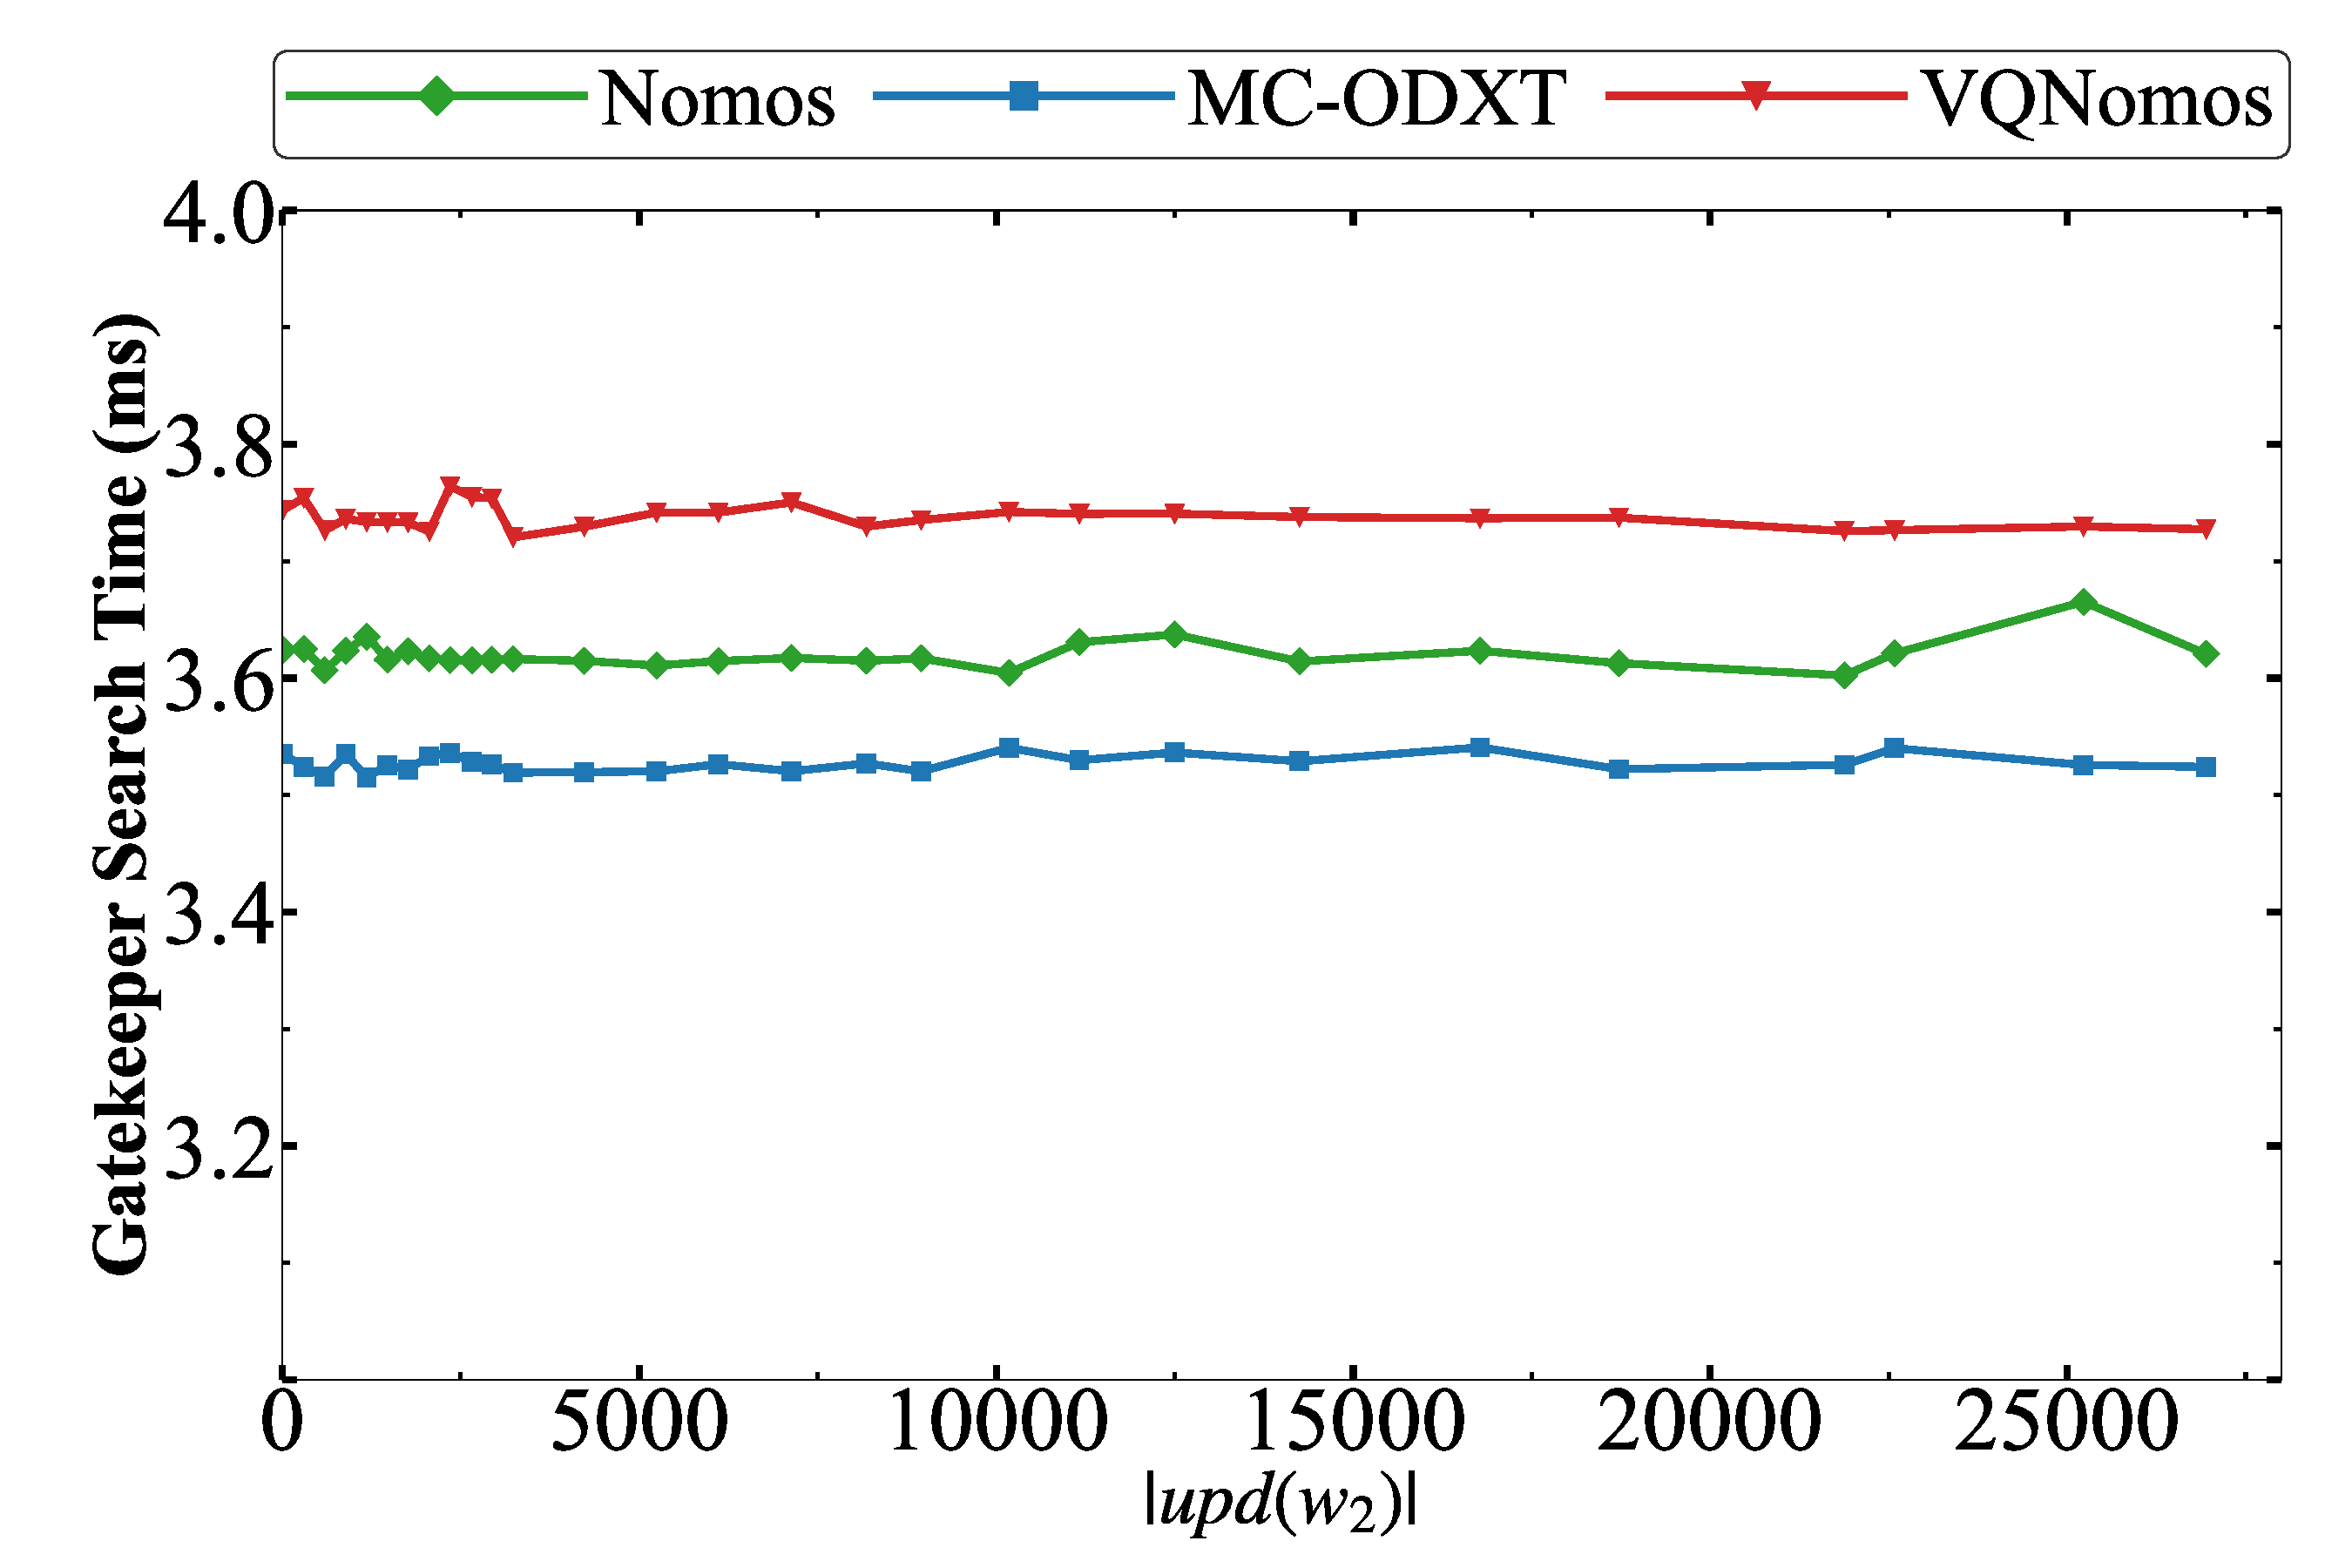
\includegraphics[width=\linewidth]
            {../figures/gatekeeper_search_time_fixed_w1_figures/Enron_gatekeeper_search_time_comparison.pdf}
        \end{subfigure}
        \caption{授权管理方搜索时间}
      \end{figure}
  \end{columns}

  \begin{exampleblock}{服务器时间增量 $< 20\%$，理论与实验高度吻合}
  \end{exampleblock}

\end{frame}

% ---- Slide: 存储开销 ----
\begin{frame}{实验结果（三）：存储开销}

  \begin{columns}[T]
    \column{0.56\textwidth}
      \begin{figure}
        \begin{subfigure}[b]{0.48\textwidth}
          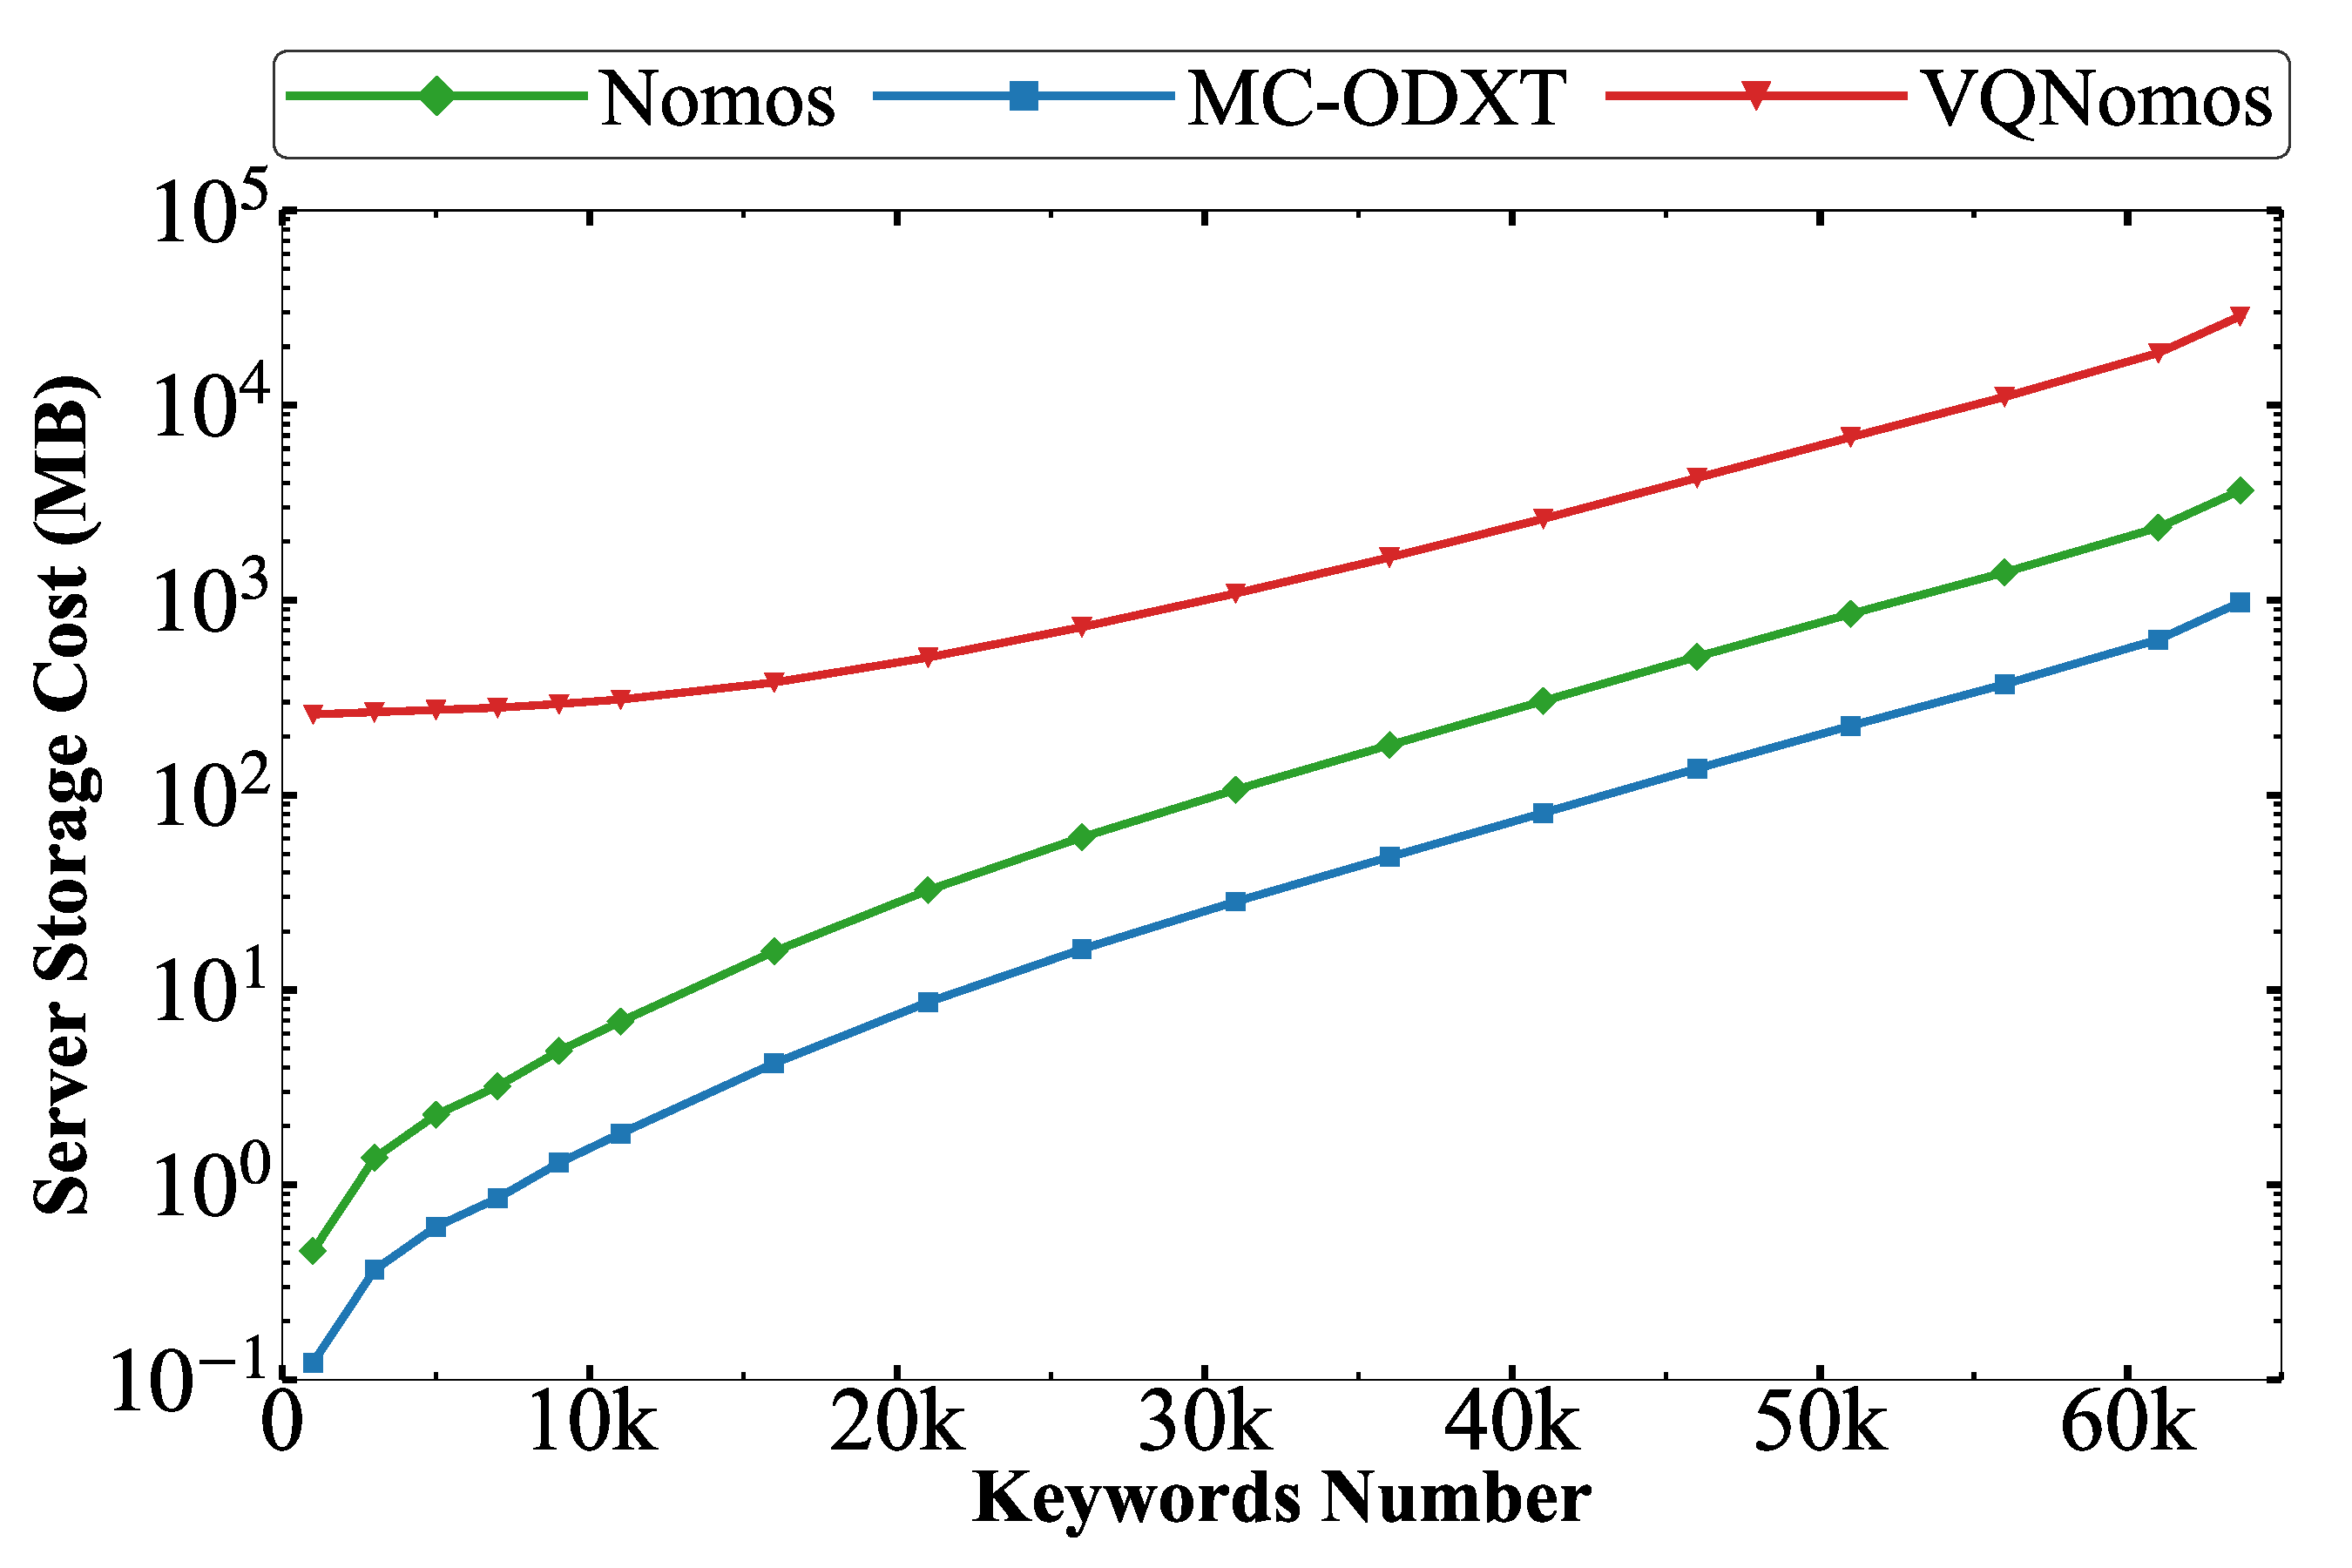
\includegraphics[width=\linewidth]
            {../figures/nomos_server_storage/Crime_server_storage_comparison.pdf}
          \caption{Crime}
        \end{subfigure}
        \hfill
        \begin{subfigure}[b]{0.48\textwidth}
          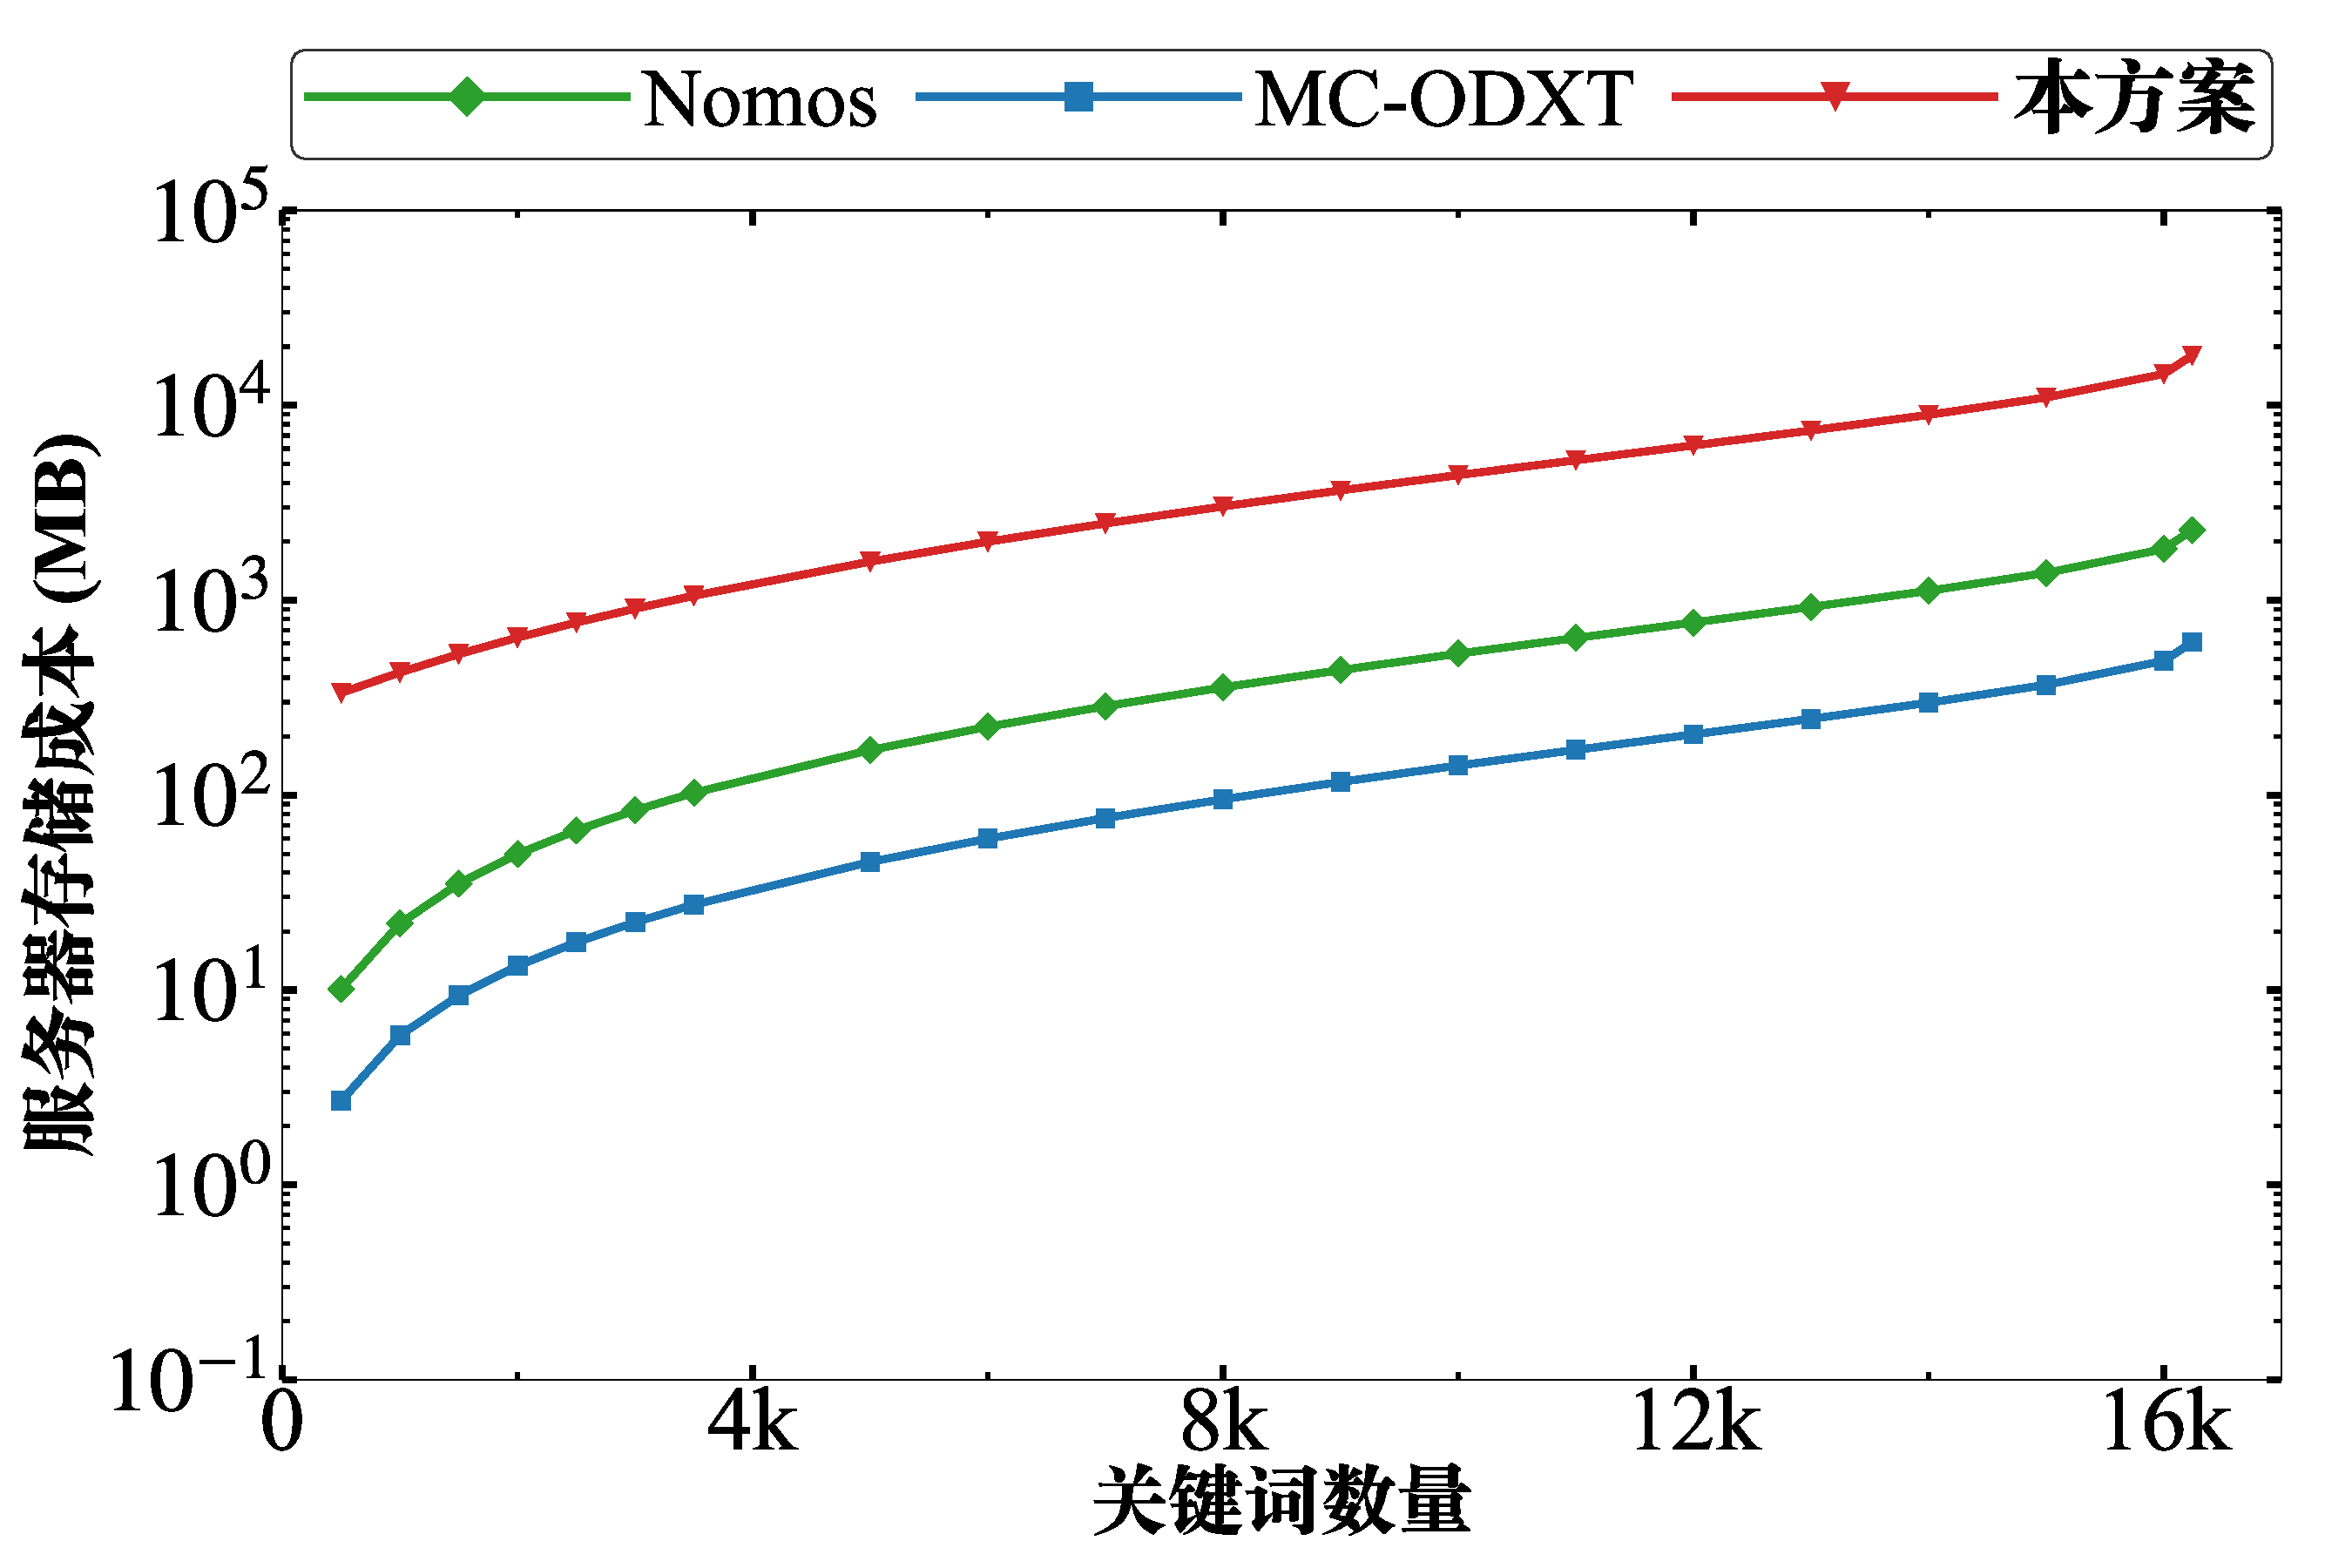
\includegraphics[width=\linewidth]
            {../figures/nomos_server_storage/Enron_server_storage_comparison.pdf}
          \caption{Enron}
        \end{subfigure}
        \caption{服务器存储开销（相对 Nomos 对比）}
      \end{figure}

    \column{0.41\textwidth}
      \begin{block}{存储汇总}
        \small
        \begin{tabular}{lll}
          \toprule
          \textbf{数据集} & \textbf{Nomos} & \textbf{本文} \\
          \midrule
          Crime & 765\,MB & 7.4\,GB \\
          Enron & 497\,MB & 4.8\,GB \\
          Wiki  & 437\,MB & 4.2\,GB \\
          \bottomrule
        \end{tabular}
      \end{block}

      \vspace{0.4em}
      \begin{exampleblock}{分析}
        \small
        \begin{itemize}
          \item 服务器存储膨胀源于 MPos $+$ MTree 结构
          \item 渐近 $O(N\ell\lambda)$，可通过压缩优化
          \item \textbf{客户端存储增量 $< 0.1\%$}，对用户透明
        \end{itemize}
      \end{exampleblock}
  \end{columns}

\end{frame}

% ---- Slide: 通信开销 ----
\begin{frame}{实验结果（四）：通信开销}

  \begin{columns}[T]
    \column{0.56\textwidth}
      \begin{figure}
        \begin{subfigure}[b]{0.48\textwidth}
          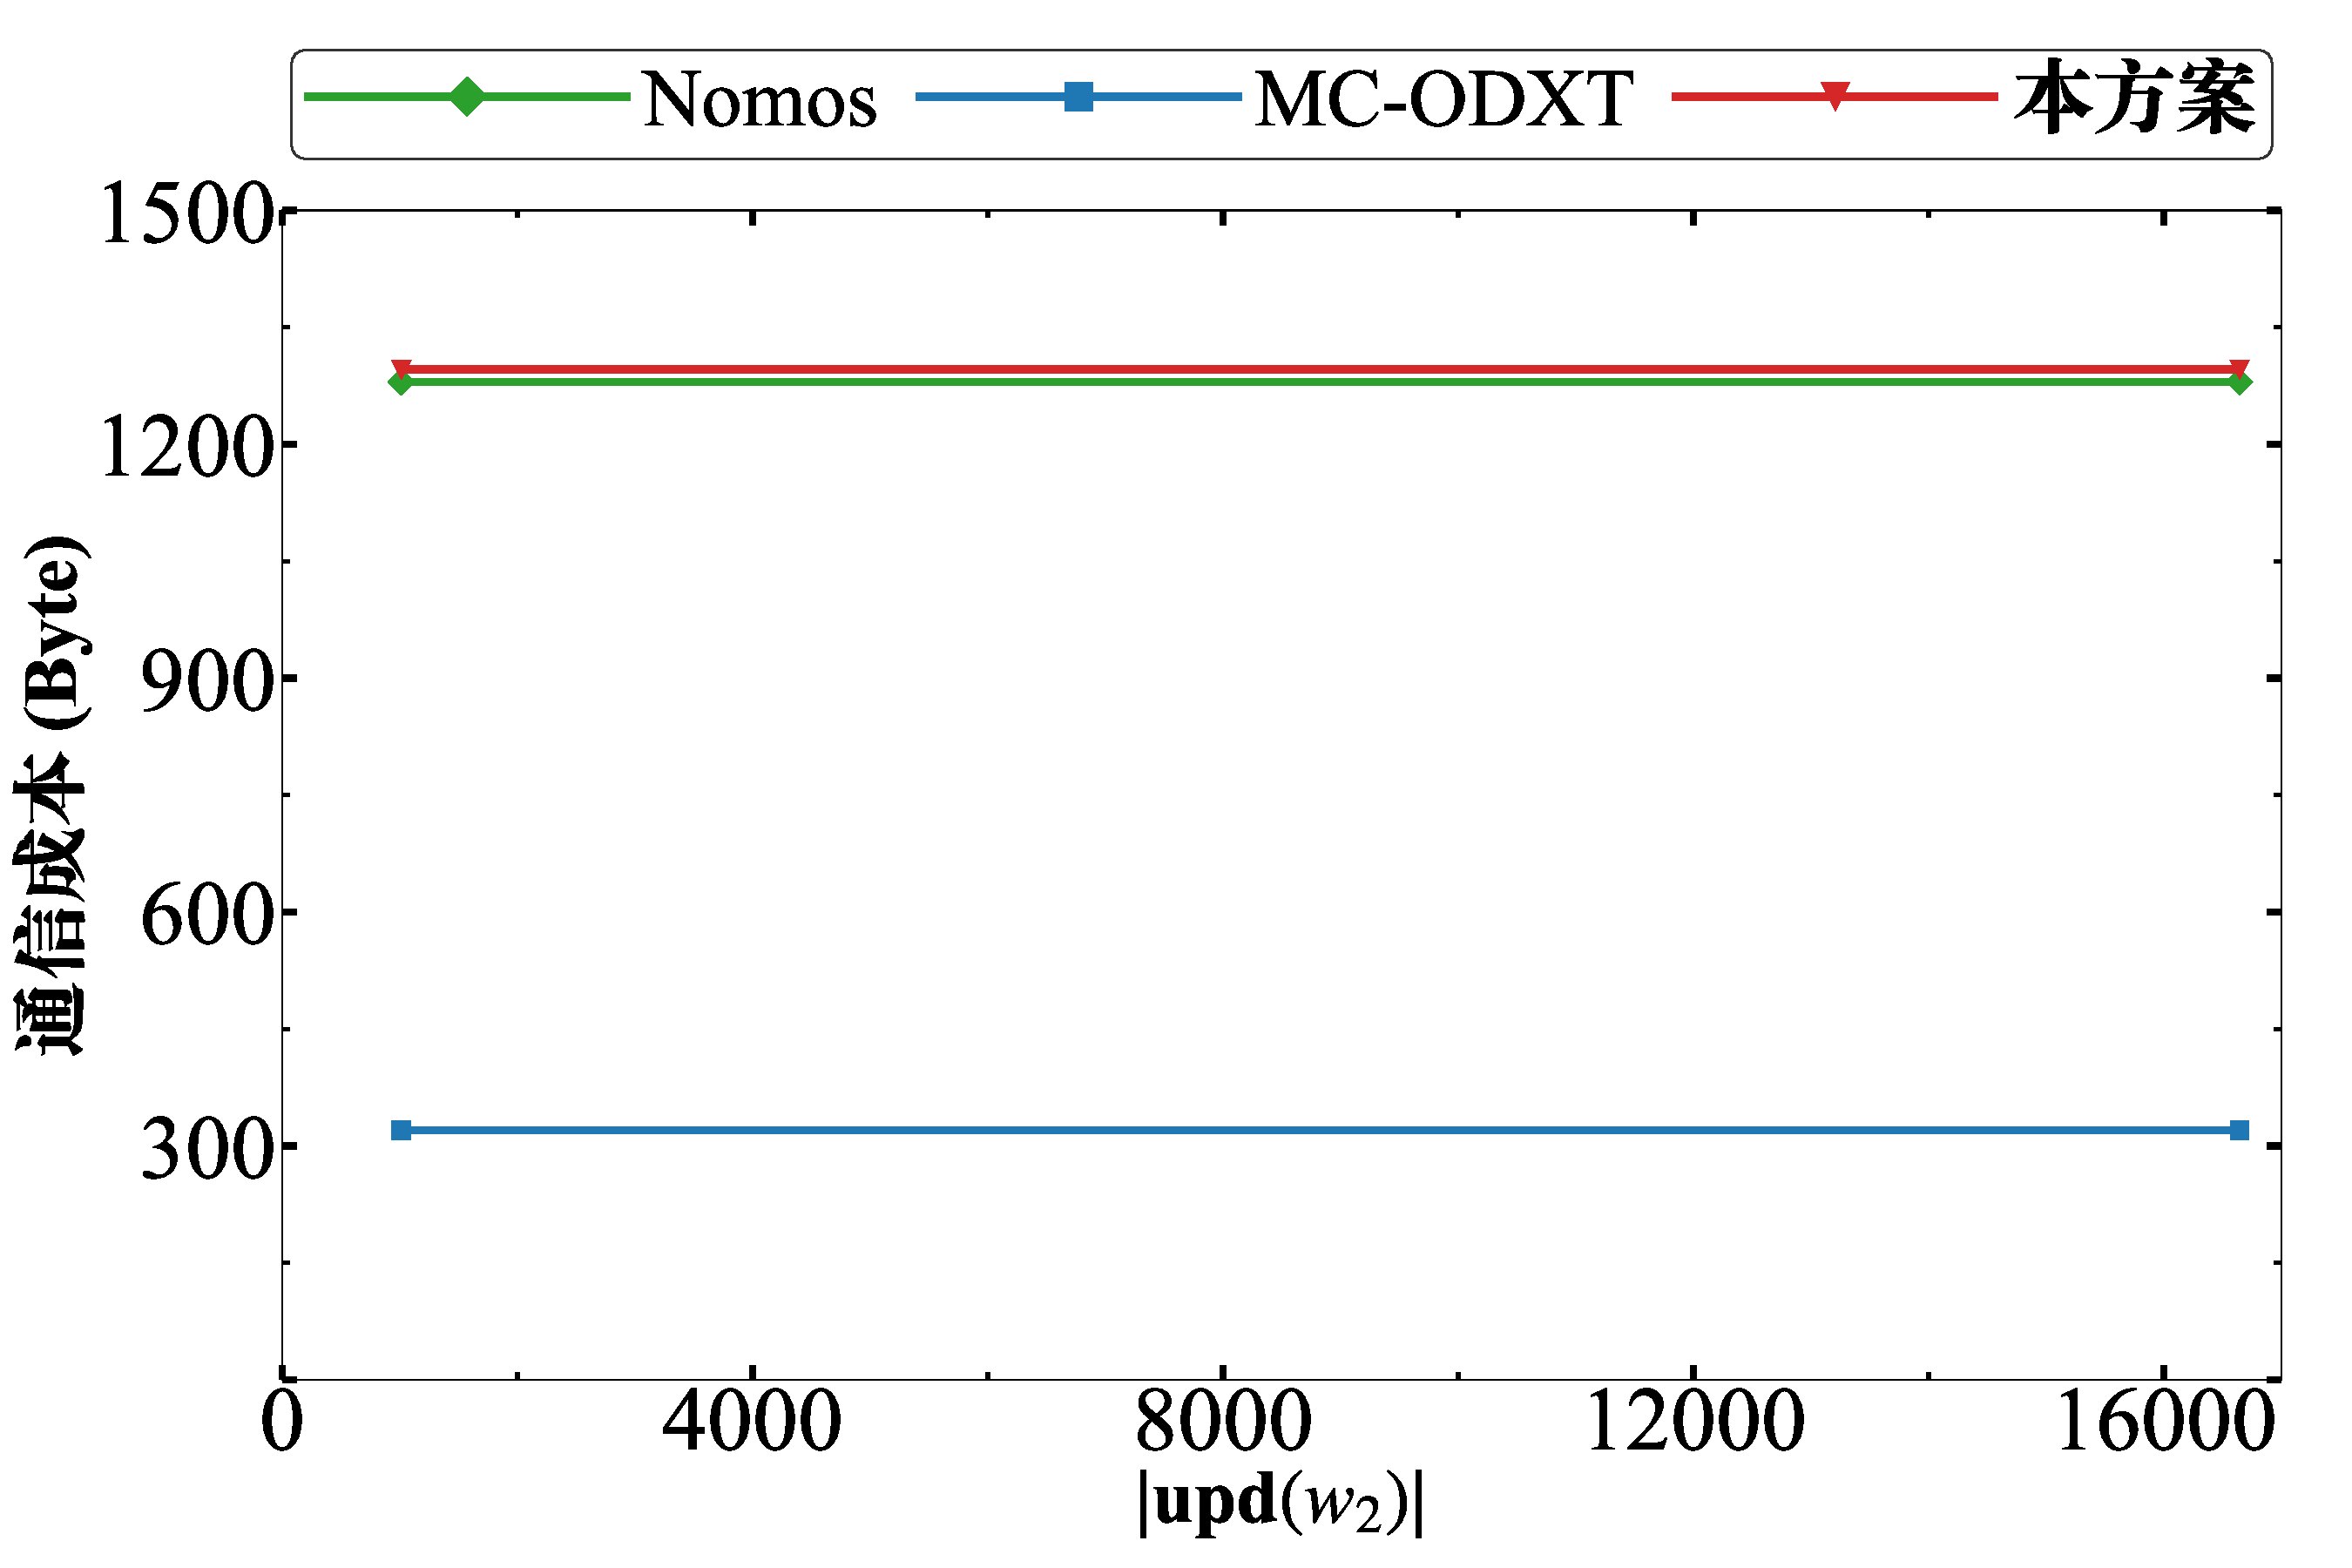
\includegraphics[width=\linewidth]
            {../figures/nomos_client_communication_w1/Crime_client_communication_comparison.pdf}
          \caption{Crime}
        \end{subfigure}
        \hfill
        \begin{subfigure}[b]{0.48\textwidth}
          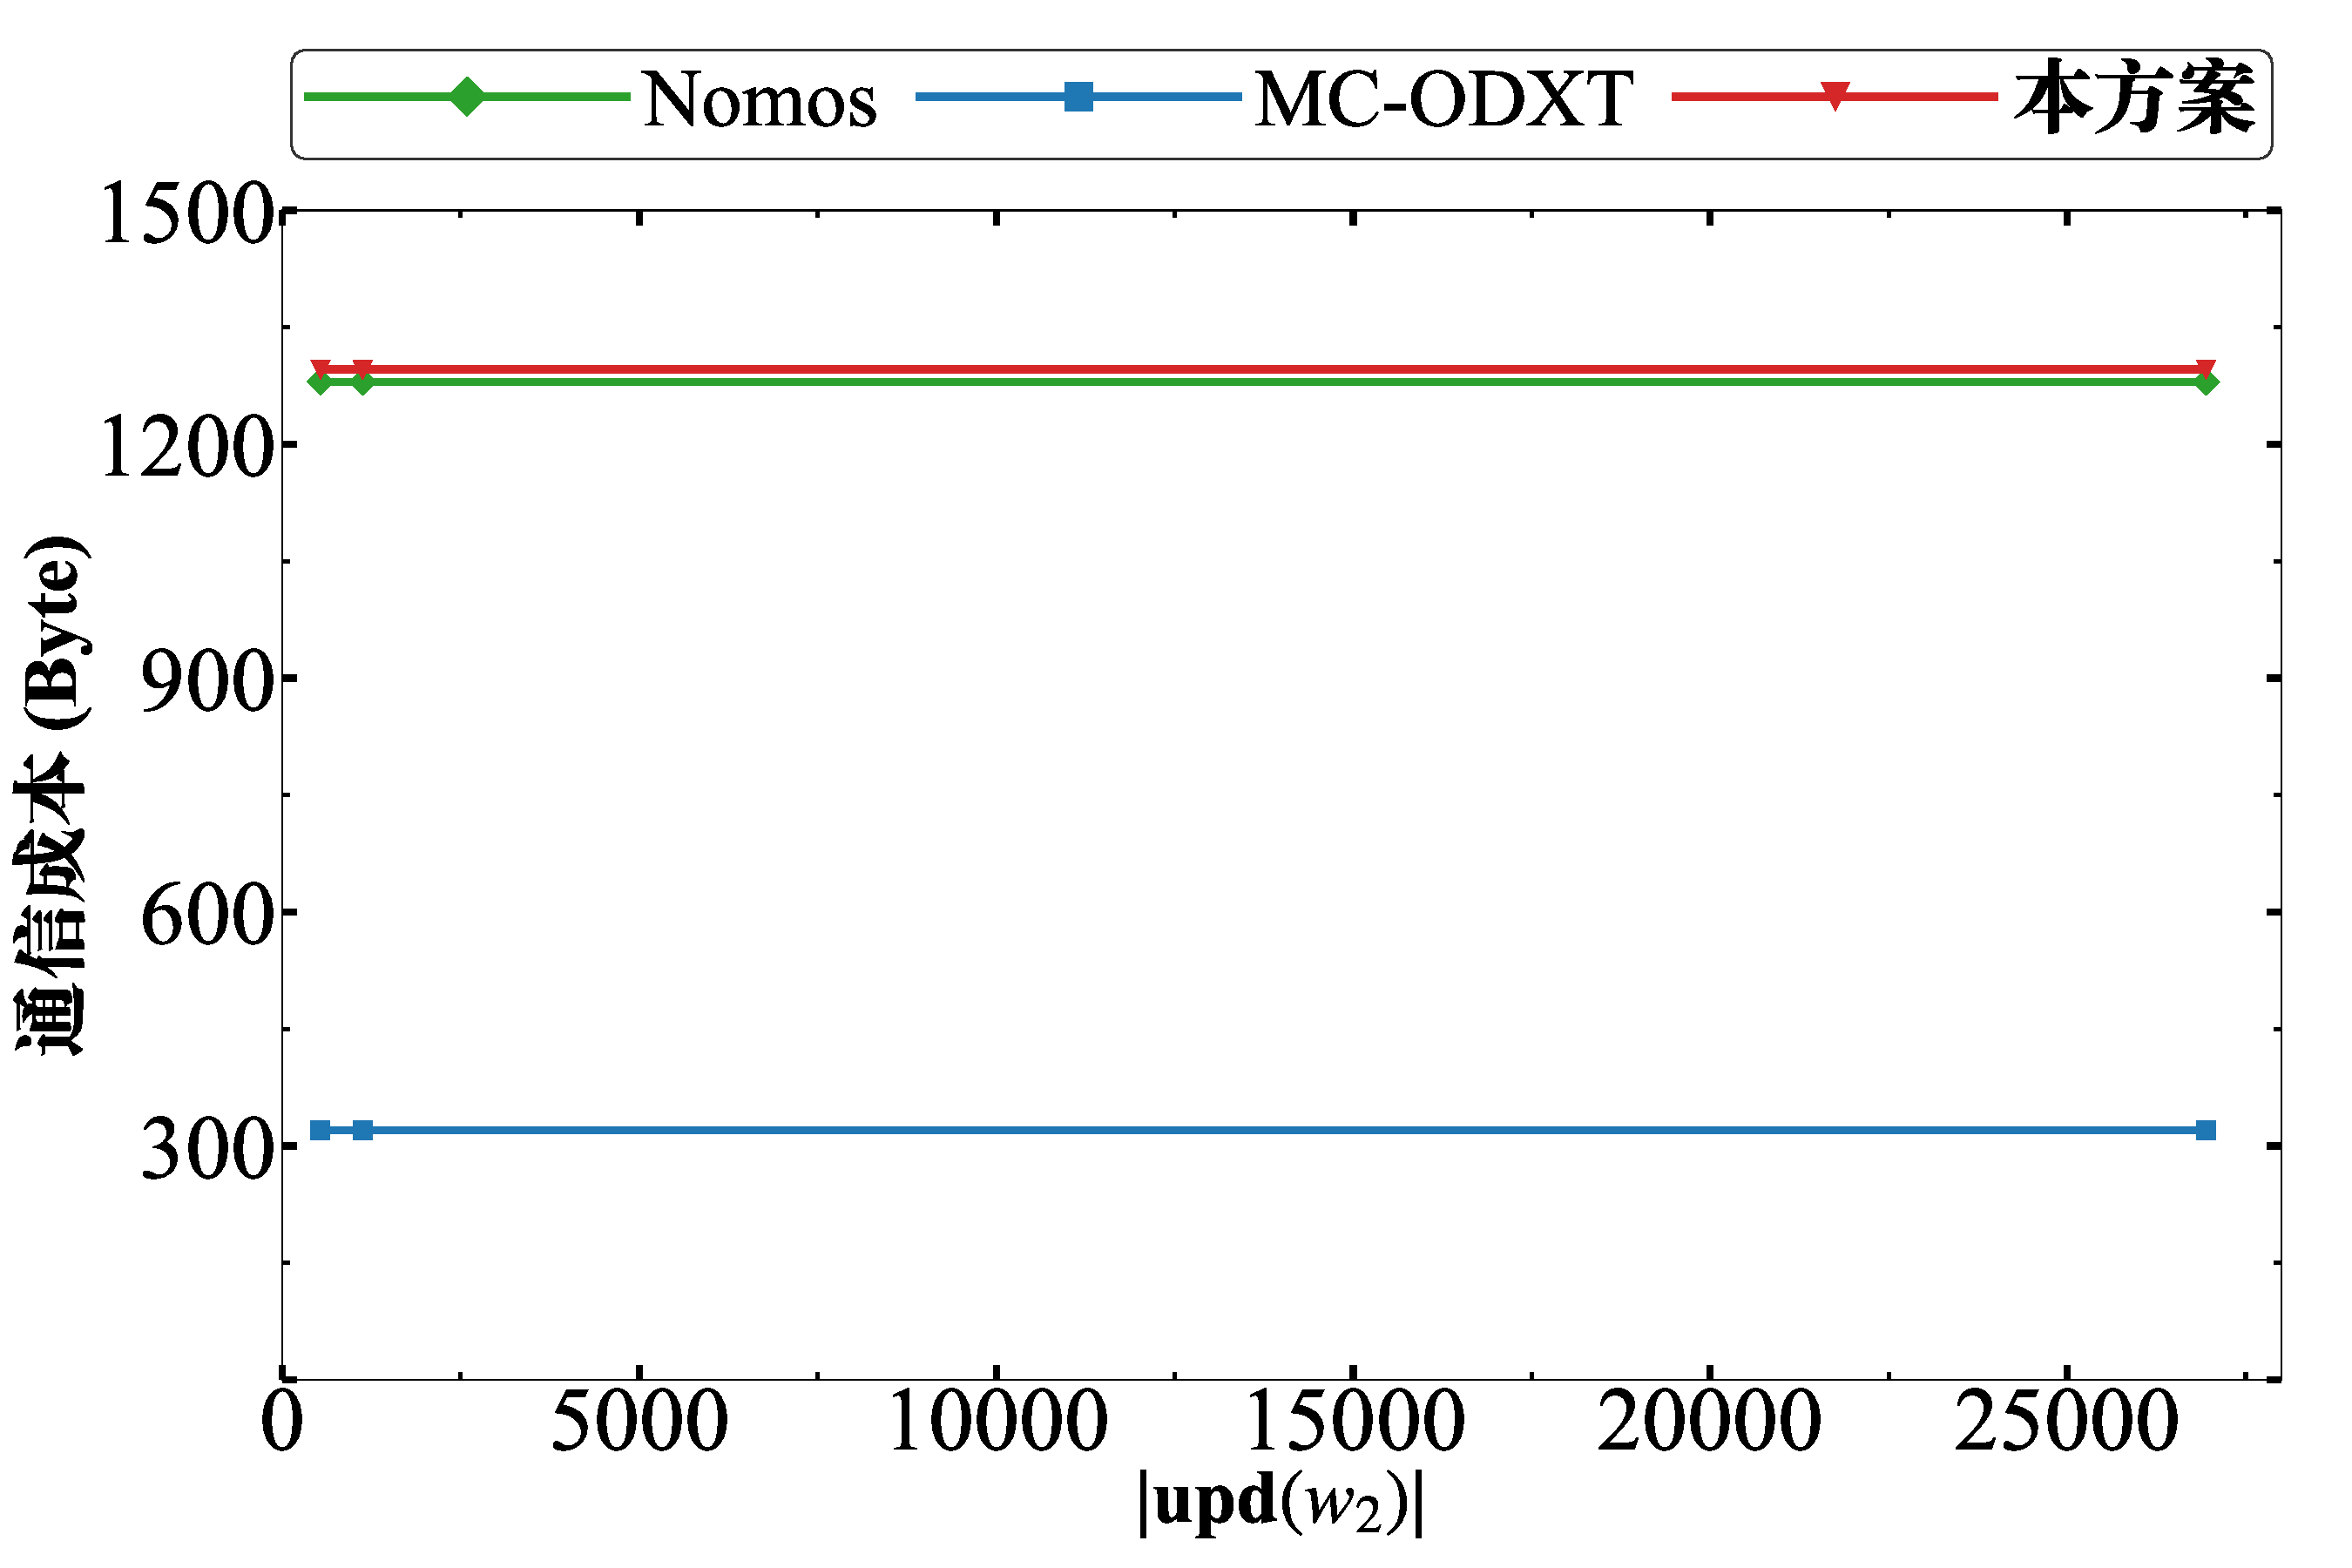
\includegraphics[width=\linewidth]
            {../figures/nomos_client_communication_w1/Enron_client_communication_comparison.pdf}
          \caption{Enron}
        \end{subfigure}
        \caption{客户端通信开销（相对 Nomos 对比）}
      \end{figure}

    \column{0.41\textwidth}
      \begin{block}{通信开销分析}
        \small
        \begin{itemize}
          \item \textbf{客户端上传增量}：$< 0.2\%$\\
                （仅版本号 8\,B + 采样索引 8\,B）
          \item \textbf{服务器下发增量}：\\
                $O(k(\log M + \log \ell))$ 哈希值
          \item 选择性开封将单条关系通信\\
                从 $O(\ell|\mathbb{G}|)$ 降至 $O(k(|\mathbb{G}|+\lambda\log\ell))$
        \end{itemize}
      \end{block}

      \vspace{0.3em}
      \begin{exampleblock}{综合结论}
        \small
        客户端与通信侧开销几乎可忽略，
        服务器侧存储为主要代价，
        整体轻量，适合多用户云端部署。
      \end{exampleblock}
  \end{columns}

\end{frame}
